\documentclass[twoside]{book}

% Packages required by doxygen
\usepackage{fixltx2e}
\usepackage{calc}
\usepackage{doxygen}
\usepackage[export]{adjustbox} % also loads graphicx
\usepackage{graphicx}
\usepackage[utf8]{inputenc}
\usepackage{makeidx}
\usepackage{multicol}
\usepackage{multirow}
\PassOptionsToPackage{warn}{textcomp}
\usepackage{textcomp}
\usepackage[nointegrals]{wasysym}
\usepackage[table]{xcolor}

% Font selection
\usepackage[T1]{fontenc}
\usepackage[scaled=.90]{helvet}
\usepackage{courier}
\usepackage{amssymb}
\usepackage{sectsty}
\renewcommand{\familydefault}{\sfdefault}
\allsectionsfont{%
  \fontseries{bc}\selectfont%
  \color{darkgray}%
}
\renewcommand{\DoxyLabelFont}{%
  \fontseries{bc}\selectfont%
  \color{darkgray}%
}
\newcommand{\+}{\discretionary{\mbox{\scriptsize$\hookleftarrow$}}{}{}}

% Page & text layout
\usepackage{geometry}
\geometry{%
  a4paper,%
  top=2.5cm,%
  bottom=2.5cm,%
  left=2.5cm,%
  right=2.5cm%
}
\tolerance=750
\hfuzz=15pt
\hbadness=750
\setlength{\emergencystretch}{15pt}
\setlength{\parindent}{0cm}
\setlength{\parskip}{3ex plus 2ex minus 2ex}
\makeatletter
\renewcommand{\paragraph}{%
  \@startsection{paragraph}{4}{0ex}{-1.0ex}{1.0ex}{%
    \normalfont\normalsize\bfseries\SS@parafont%
  }%
}
\renewcommand{\subparagraph}{%
  \@startsection{subparagraph}{5}{0ex}{-1.0ex}{1.0ex}{%
    \normalfont\normalsize\bfseries\SS@subparafont%
  }%
}
\makeatother

% Headers & footers
\usepackage{fancyhdr}
\pagestyle{fancyplain}
\fancyhead[LE]{\fancyplain{}{\bfseries\thepage}}
\fancyhead[CE]{\fancyplain{}{}}
\fancyhead[RE]{\fancyplain{}{\bfseries\leftmark}}
\fancyhead[LO]{\fancyplain{}{\bfseries\rightmark}}
\fancyhead[CO]{\fancyplain{}{}}
\fancyhead[RO]{\fancyplain{}{\bfseries\thepage}}
\fancyfoot[LE]{\fancyplain{}{}}
\fancyfoot[CE]{\fancyplain{}{}}
\fancyfoot[RE]{\fancyplain{}{\bfseries\scriptsize Generated by Doxygen }}
\fancyfoot[LO]{\fancyplain{}{\bfseries\scriptsize Generated by Doxygen }}
\fancyfoot[CO]{\fancyplain{}{}}
\fancyfoot[RO]{\fancyplain{}{}}
\renewcommand{\footrulewidth}{0.4pt}
\renewcommand{\chaptermark}[1]{%
  \markboth{#1}{}%
}
\renewcommand{\sectionmark}[1]{%
  \markright{\thesection\ #1}%
}

% Indices & bibliography
\usepackage{natbib}
\usepackage[titles]{tocloft}
\setcounter{tocdepth}{3}
\setcounter{secnumdepth}{5}
\makeindex

% Hyperlinks (required, but should be loaded last)
\usepackage{ifpdf}
\ifpdf
  \usepackage[pdftex,pagebackref=true]{hyperref}
\else
  \usepackage[ps2pdf,pagebackref=true]{hyperref}
\fi
\hypersetup{%
  colorlinks=true,%
  linkcolor=blue,%
  citecolor=blue,%
  unicode%
}

% Custom commands
\newcommand{\clearemptydoublepage}{%
  \newpage{\pagestyle{empty}\cleardoublepage}%
}

\usepackage{caption}
\captionsetup{labelsep=space,justification=centering,font={bf},singlelinecheck=off,skip=4pt,position=top}

%===== C O N T E N T S =====

\begin{document}

% Titlepage & ToC
\hypersetup{pageanchor=false,
             bookmarksnumbered=true,
             pdfencoding=unicode
            }
\pagenumbering{alph}
\begin{titlepage}
\vspace*{7cm}
\begin{center}%
{\Large Ble\+Serial\+Peripheral\+RK }\\
\vspace*{1cm}
{\large Generated by Doxygen 1.8.14}\\
\end{center}
\end{titlepage}
\clearemptydoublepage
\pagenumbering{roman}
\tableofcontents
\clearemptydoublepage
\pagenumbering{arabic}
\hypersetup{pageanchor=true}

%--- Begin generated contents ---
\chapter{Ble\+Serial\+Peripheral\+RK}
\label{index}\hypertarget{index}{}{\itshape Library to simplify using B\+LE U\+A\+RT peripheral mode on Gen 3 devices}

\subsection*{Introduction}

Particle Gen 3 devices (Argon, Boron, Xenon) running Device OS 1.\+3.\+0-\/rc.\+1 and later have support for B\+LE (Bluetooth Low Entergy) in central and peripheral roles.

Nordic Semiconductor created a U\+A\+RT peripheral protocol to allow central devices (like mobile phones) to connect to a B\+LE device and read U\+A\+R\+T-\/like data streams. This is supported not only by the n\+RF Toolbox app, but also some other apps like the Adafruit Bluefruit app.

There is \href{https://docs.particle.io/tutorials/device-os/bluetooth-le/#uart-peripheral}{\tt a code example in the docs}, however this class encapsulates the B\+LE stuff and makes a Serial-\/like interface to it. Among the benefits\+:


\begin{DoxyItemize}
\item Reading is easy using standard functions like read(), read\+Until(), read\+String(), etc. like you can from Serial, Serial1, etc..
\item Writing is easy and buffered, allowing not only write() to write a byte, but also all of the variations of print(), println(), printf(), printlnf(), etc. that are available when using Serial, etc..
\item All of the B\+LE stuff is encapsulated so you don\textquotesingle{}t have to worry about it.
\end{DoxyItemize}

\subsection*{Example}

There is one example in 1-\/simple-\/\+Ble\+Serial\+Peripheral\+RK\+:


\begin{DoxyCode}
#include "BleSerialPeripheralRK.h"

SerialLogHandler logHandler;

SYSTEM\_THREAD(ENABLED);

// First parameter is the transmit buffer size, second parameter is the receive buffer size
BleSerialPeripheralStatic<32, 256> bleSerial;

const unsigned long TRANSMIT\_PERIOD\_MS = 2000;
unsigned long lastTransmit = 0;
int counter = 0;


void setup() \{
    Serial.begin();

    // This must be called from setup()!
    bleSerial.setup();

    // If you don't have any other services to advertise, just call advertise().
    // Otherwise, call getServiceUuid() to get the serial service UUID and add that to your
    // custom advertising data payload and call BLE.advertise() yourself with all of your necessary
    // services added.
    bleSerial.advertise();
\}

void loop() \{
    // This must be called from loop() on every call to loop.
    bleSerial.loop();

    // Print out anything we receive
    if(bleSerial.available()) \{
        String s = bleSerial.readString();

        Log.info("received: %s", s.c\_str());
    \}

    if (millis() - lastTransmit >= TRANSMIT\_PERIOD\_MS) \{
        lastTransmit = millis();

        // Every two seconds, send something to the other side
        bleSerial.printlnf("testing %d", ++counter);
        Log.info("counter=%d", counter);
    \}
\}
\end{DoxyCode}


Among the important things\+:

You normally instantiate a \mbox{\hyperlink{class_ble_serial_peripheral_static}{Ble\+Serial\+Peripheral\+Static}} object as a global variable. The first number in the $<$$>$ is the transmit buffer size and the second is the receive buffer size.


\begin{DoxyCode}
// First parameter is the transmit buffer size, second parameter is the receive buffer size
BleSerialPeripheralStatic<256, 256> bleSerial;
\end{DoxyCode}


Because the data is buffered and only sent from loop() the transmit buffer must be larger than the amount of data you intend to sent at once, or the maximum data that will accumulate between calls to loop.

Likewise, since data is read from loop but received asynchronously by B\+LE, you must have a receive buffer that is large enough to hold any data between times you will be processing it from your loop function.

If there is a data overflow situation, the data is discarded.

Be sure to call this from your setup() function.


\begin{DoxyCode}
bleSerial.setup();
\end{DoxyCode}


If you are only using B\+LE U\+A\+RT you can call\+:


\begin{DoxyCode}
bleSerial.advertise();
\end{DoxyCode}


If you are advertising multiple services, instead call {\ttfamily ble\+Serial.\+get\+Service\+Uuid()} to get the U\+A\+RT serial U\+U\+ID and add it with your own services\+:


\begin{DoxyCode}
BleAdvertisingData data;
data.appendServiceUUID(bleSerial.getServiceUuid());
// append your own service UUIDs here
BLE.advertise(&data);
\end{DoxyCode}


Be sure to call this from loop, as often as possible.


\begin{DoxyCode}
bleSerial.loop();
\end{DoxyCode}


In this example we used {\ttfamily ble\+Serial.\+read\+String()} but there are many method of the \mbox{\hyperlink{class_stream}{Stream}} class to read. Beware of blocking, however. If you are waiting to read a string, you won\textquotesingle{}t be calling {\ttfamily ble\+Serial.\+loop()} and data won\textquotesingle{}t be transmitted during that time.

Finally, you can print to B\+LE serial using all of the standard \mbox{\hyperlink{class_stream}{Stream}} methods. The example uses {\ttfamily ble\+Serial.\+printlnf()} to print a line using {\ttfamily sprintf} formatting. 
\chapter{Hierarchical Index}
\section{Class Hierarchy}
This inheritance list is sorted roughly, but not completely, alphabetically\+:\begin{DoxyCompactList}
\item \contentsline{section}{Ble\+Serial\+Peripheral\+Lock}{\pageref{class_ble_serial_peripheral_lock}}{}
\item \contentsline{section}{Print}{\pageref{class_print}}{}
\begin{DoxyCompactList}
\item \contentsline{section}{Stream}{\pageref{class_stream}}{}
\begin{DoxyCompactList}
\item \contentsline{section}{Ble\+Serial\+Peripheral\+Base}{\pageref{class_ble_serial_peripheral_base}}{}
\begin{DoxyCompactList}
\item \contentsline{section}{Ble\+Serial\+Peripheral\+Static$<$ T\+X\+\_\+\+B\+U\+F\+\_\+\+S\+I\+ZE, R\+X\+\_\+\+B\+U\+F\+\_\+\+S\+I\+ZE $>$}{\pageref{class_ble_serial_peripheral_static}}{}
\end{DoxyCompactList}
\end{DoxyCompactList}
\end{DoxyCompactList}
\item \contentsline{section}{Ring\+Buffer$<$ T $>$}{\pageref{class_ring_buffer}}{}
\item \contentsline{section}{Ring\+Buffer$<$ uint8\+\_\+t $>$}{\pageref{class_ring_buffer}}{}
\end{DoxyCompactList}

\chapter{Data Structure Index}
\section{Data Structures}
Here are the data structures with brief descriptions\+:\begin{DoxyCompactList}
\item\contentsline{section}{\mbox{\hyperlink{class_ble_serial_peripheral_base}{Ble\+Serial\+Peripheral\+Base}} \\*Main class for B\+LE U\+A\+RT funtionality }{\pageref{class_ble_serial_peripheral_base}}{}
\item\contentsline{section}{\mbox{\hyperlink{class_ble_serial_peripheral_lock}{Ble\+Serial\+Peripheral\+Lock}} \\*Class to lock and unlock the tx mutex automatically. Allocate this object on the stack so when it goes out of scope the mutex will always be released }{\pageref{class_ble_serial_peripheral_lock}}{}
\item\contentsline{section}{\mbox{\hyperlink{class_ble_serial_peripheral_static}{Ble\+Serial\+Peripheral\+Static$<$ T\+X\+\_\+\+B\+U\+F\+\_\+\+S\+I\+Z\+E, R\+X\+\_\+\+B\+U\+F\+\_\+\+S\+I\+Z\+E $>$}} \\*Ble\+Serial\+Peripheral with static buffers. This is the object you will normally create, as a global variable }{\pageref{class_ble_serial_peripheral_static}}{}
\item\contentsline{section}{\mbox{\hyperlink{class_print}{Print}} \\*Class for printing to a stream or file }{\pageref{class_print}}{}
\item\contentsline{section}{\mbox{\hyperlink{class_ring_buffer}{Ring\+Buffer$<$ T $>$}} \\*Thread and interrupt-\/safe (with caveats) circular buffer (ring buffer) class }{\pageref{class_ring_buffer}}{}
\item\contentsline{section}{\mbox{\hyperlink{class_stream}{Stream}} \\*Arduino/\+Wiring \mbox{\hyperlink{class_stream}{Stream}} Class }{\pageref{class_stream}}{}
\end{DoxyCompactList}

\chapter{File Index}
\section{File List}
Here is a list of all documented files with brief descriptions\+:\begin{DoxyCompactList}
\item\contentsline{section}{docs/src/\mbox{\hyperlink{spark__wiring__print_8h}{spark\+\_\+wiring\+\_\+print.\+h}} \\*Header for spark\+\_\+wiring\+\_\+print.\+c module }{\pageref{spark__wiring__print_8h}}{}
\item\contentsline{section}{docs/src/\mbox{\hyperlink{spark__wiring__stream_8h}{spark\+\_\+wiring\+\_\+stream.\+h}} \\*Header for spark\+\_\+wiring\+\_\+stream.\+c module }{\pageref{spark__wiring__stream_8h}}{}
\item\contentsline{section}{src/{\bfseries Ble\+Serial\+Peripheral\+R\+K.\+h} }{\pageref{_ble_serial_peripheral_r_k_8h}}{}
\item\contentsline{section}{src/{\bfseries Ring\+Buffer.\+h} }{\pageref{_ring_buffer_8h}}{}
\end{DoxyCompactList}

\chapter{Data Structure Documentation}
\hypertarget{class_ble_serial_peripheral_base}{}\section{Ble\+Serial\+Peripheral\+Base Class Reference}
\label{class_ble_serial_peripheral_base}\index{Ble\+Serial\+Peripheral\+Base@{Ble\+Serial\+Peripheral\+Base}}


Main class for B\+LE U\+A\+RT funtionality.  




{\ttfamily \#include $<$Ble\+Serial\+Peripheral\+R\+K.\+h$>$}

Inheritance diagram for Ble\+Serial\+Peripheral\+Base\+:\begin{figure}[H]
\begin{center}
\leavevmode
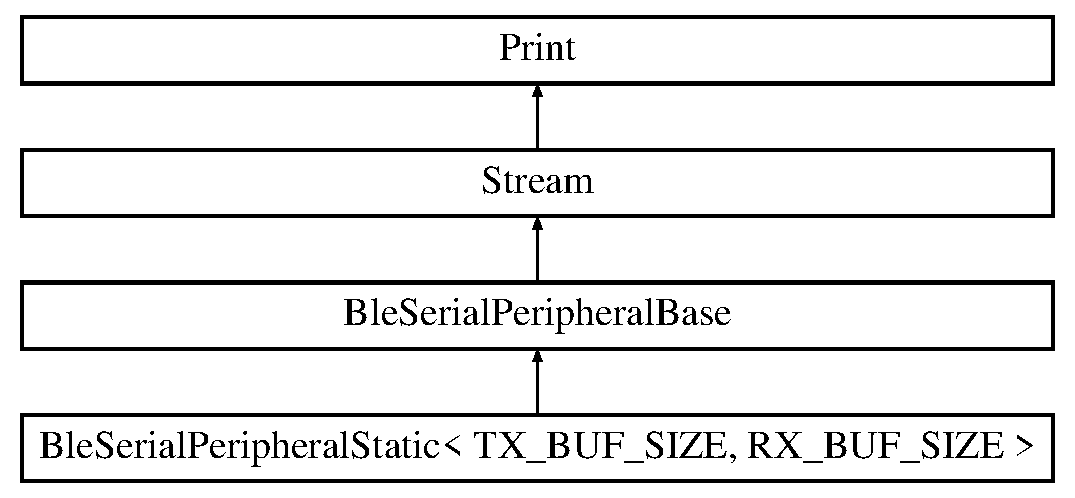
\includegraphics[height=4.000000cm]{class_ble_serial_peripheral_base}
\end{center}
\end{figure}
\subsection*{Public Member Functions}
\begin{DoxyCompactItemize}
\item 
\mbox{\hyperlink{class_ble_serial_peripheral_base_a1c1811adb8b03e7c0cb6e5f6c0a42fab}{Ble\+Serial\+Peripheral\+Base}} (uint8\+\_\+t $\ast$tx\+Buf, size\+\_\+t tx\+Buf\+Size, uint8\+\_\+t $\ast$rx\+Buf, size\+\_\+t rx\+Buf\+Size)
\begin{DoxyCompactList}\small\item\em Construct an object with passed-\/in buffers. \end{DoxyCompactList}\item 
virtual \mbox{\hyperlink{class_ble_serial_peripheral_base_ab693dd8a00b3af5ed375d68647bb4712}{$\sim$\+Ble\+Serial\+Peripheral\+Base}} ()
\begin{DoxyCompactList}\small\item\em Destructor. \end{DoxyCompactList}\item 
\mbox{\Hypertarget{class_ble_serial_peripheral_base_a01072243aecf86ea5030019a6e900fbb}\label{class_ble_serial_peripheral_base_a01072243aecf86ea5030019a6e900fbb}} 
void \mbox{\hyperlink{class_ble_serial_peripheral_base_a01072243aecf86ea5030019a6e900fbb}{setup}} ()
\begin{DoxyCompactList}\small\item\em You must call this from \mbox{\hyperlink{class_ble_serial_peripheral_base_a01072243aecf86ea5030019a6e900fbb}{setup()}} to initialize the object. \end{DoxyCompactList}\item 
\mbox{\Hypertarget{class_ble_serial_peripheral_base_a441dc005092891279967444cb2dc2ff2}\label{class_ble_serial_peripheral_base_a441dc005092891279967444cb2dc2ff2}} 
void \mbox{\hyperlink{class_ble_serial_peripheral_base_a441dc005092891279967444cb2dc2ff2}{loop}} ()
\begin{DoxyCompactList}\small\item\em You must call this from \mbox{\hyperlink{class_ble_serial_peripheral_base_a441dc005092891279967444cb2dc2ff2}{loop()}} to process outgoing data. \end{DoxyCompactList}\item 
void \mbox{\hyperlink{class_ble_serial_peripheral_base_a870258aa62e285cc0e2717476ae51145}{advertise}} ()
\begin{DoxyCompactList}\small\item\em Call this to advertise the B\+LE U\+A\+RT service. \end{DoxyCompactList}\item 
Ble\+Uuid \mbox{\hyperlink{class_ble_serial_peripheral_base_a0457f2495023d47468a2f5b1964c0233}{get\+Service\+Uuid}} () const
\begin{DoxyCompactList}\small\item\em Get the service U\+U\+ID for the U\+A\+RT service. \end{DoxyCompactList}\item 
void \mbox{\hyperlink{class_ble_serial_peripheral_base_a4dac5d6f8efb72b1df255e942a054560}{lock}} ()
\begin{DoxyCompactList}\small\item\em Obtain a mutex lock on the TX buffer. \end{DoxyCompactList}\item 
void \mbox{\hyperlink{class_ble_serial_peripheral_base_ab6c9183c6e2d42babe005b222b984d03}{unlock}} ()
\begin{DoxyCompactList}\small\item\em Release the mutex lock on the TX buffer. \end{DoxyCompactList}\item 
\mbox{\Hypertarget{class_ble_serial_peripheral_base_a946cc56677f03db99de9409851427941}\label{class_ble_serial_peripheral_base_a946cc56677f03db99de9409851427941}} 
virtual int \mbox{\hyperlink{class_ble_serial_peripheral_base_a946cc56677f03db99de9409851427941}{available}} ()
\begin{DoxyCompactList}\small\item\em Override for \mbox{\hyperlink{class_stream}{Stream}} class, returns the number of bytes that can be read right now. \end{DoxyCompactList}\item 
\mbox{\Hypertarget{class_ble_serial_peripheral_base_a4933bc35d89028134597b46315806ce4}\label{class_ble_serial_peripheral_base_a4933bc35d89028134597b46315806ce4}} 
virtual int \mbox{\hyperlink{class_ble_serial_peripheral_base_a4933bc35d89028134597b46315806ce4}{read}} ()
\begin{DoxyCompactList}\small\item\em Override for the \mbox{\hyperlink{class_stream}{Stream}} class, reads a byte of data from the input ring buffer. \end{DoxyCompactList}\item 
\mbox{\Hypertarget{class_ble_serial_peripheral_base_a6ba8319f3b1a69c96c4e8b3f8dde5bbc}\label{class_ble_serial_peripheral_base_a6ba8319f3b1a69c96c4e8b3f8dde5bbc}} 
virtual int \mbox{\hyperlink{class_ble_serial_peripheral_base_a6ba8319f3b1a69c96c4e8b3f8dde5bbc}{peek}} ()
\begin{DoxyCompactList}\small\item\em Override for the \mbox{\hyperlink{class_stream}{Stream}} class, reads a byte of data, but leaves it in the buffer so \mbox{\hyperlink{class_ble_serial_peripheral_base_a4933bc35d89028134597b46315806ce4}{read()}} will get the same byte of data. \end{DoxyCompactList}\item 
\mbox{\Hypertarget{class_ble_serial_peripheral_base_a27e43dcfd3cb2edee33b19ba9017ad7f}\label{class_ble_serial_peripheral_base_a27e43dcfd3cb2edee33b19ba9017ad7f}} 
virtual void \mbox{\hyperlink{class_ble_serial_peripheral_base_a27e43dcfd3cb2edee33b19ba9017ad7f}{flush}} ()
\begin{DoxyCompactList}\small\item\em Override for the \mbox{\hyperlink{class_stream}{Stream}} class. Currently does nothing. \end{DoxyCompactList}\item 
virtual size\+\_\+t \mbox{\hyperlink{class_ble_serial_peripheral_base_ac041322685f26d921f60d01a2ed99e83}{write}} (uint8\+\_\+t data)
\begin{DoxyCompactList}\small\item\em Virtual override from the \mbox{\hyperlink{class_print}{Print}} class. Writes a byte of data. \end{DoxyCompactList}\item 
size\+\_\+t \mbox{\hyperlink{class_ble_serial_peripheral_base_a97cee829a39ff3a62e3108f05fba64d8}{get\+Rx\+Lost}} () const
\item 
\mbox{\Hypertarget{class_ble_serial_peripheral_base_af2dc5ee170da6783176ce6c96456fdb4}\label{class_ble_serial_peripheral_base_af2dc5ee170da6783176ce6c96456fdb4}} 
void \mbox{\hyperlink{class_ble_serial_peripheral_base_af2dc5ee170da6783176ce6c96456fdb4}{clear\+Rx\+Lost}} ()
\begin{DoxyCompactList}\small\item\em Clears the rx\+Lost counter. \end{DoxyCompactList}\item 
size\+\_\+t \mbox{\hyperlink{class_ble_serial_peripheral_base_a09c779ad7767bc195687c525548127d9}{get\+Tx\+Lost}} () const
\item 
\mbox{\Hypertarget{class_ble_serial_peripheral_base_a3f7273afa5985d6df935b530d9550b6c}\label{class_ble_serial_peripheral_base_a3f7273afa5985d6df935b530d9550b6c}} 
void \mbox{\hyperlink{class_ble_serial_peripheral_base_a3f7273afa5985d6df935b530d9550b6c}{clear\+Tx\+Lost}} ()
\begin{DoxyCompactList}\small\item\em Clears the tx\+Lost counter. \end{DoxyCompactList}\item 
\mbox{\Hypertarget{class_ble_serial_peripheral_base_aa4ca5408c166841e1fd5ea9aa3a1c4a5}\label{class_ble_serial_peripheral_base_aa4ca5408c166841e1fd5ea9aa3a1c4a5}} 
size\+\_\+t \mbox{\hyperlink{class_ble_serial_peripheral_base_aa4ca5408c166841e1fd5ea9aa3a1c4a5}{get\+Tx\+Max\+Write}} () const
\begin{DoxyCompactList}\small\item\em Get the maximum chunk size to send. The default is 236 bytes. \end{DoxyCompactList}\item 
void \mbox{\hyperlink{class_ble_serial_peripheral_base_a454bb53617c96d564f3e20d13765de9f}{set\+Tx\+Max\+Write}} (size\+\_\+t value)
\begin{DoxyCompactList}\small\item\em Set the maximum chunk size to send. \end{DoxyCompactList}\end{DoxyCompactItemize}


\subsection{Detailed Description}
Main class for B\+LE U\+A\+RT funtionality. 

Normally you\textquotesingle{}ll instantiate a \mbox{\hyperlink{class_ble_serial_peripheral_static}{Ble\+Serial\+Peripheral\+Static}} as a global variable instead of using this class.

You can only have one instance of this object per device!

Note\+: This method subclasses \mbox{\hyperlink{class_stream}{Stream}}. 

\subsection{Constructor \& Destructor Documentation}
\mbox{\Hypertarget{class_ble_serial_peripheral_base_a1c1811adb8b03e7c0cb6e5f6c0a42fab}\label{class_ble_serial_peripheral_base_a1c1811adb8b03e7c0cb6e5f6c0a42fab}} 
\index{Ble\+Serial\+Peripheral\+Base@{Ble\+Serial\+Peripheral\+Base}!Ble\+Serial\+Peripheral\+Base@{Ble\+Serial\+Peripheral\+Base}}
\index{Ble\+Serial\+Peripheral\+Base@{Ble\+Serial\+Peripheral\+Base}!Ble\+Serial\+Peripheral\+Base@{Ble\+Serial\+Peripheral\+Base}}
\subsubsection{\texorpdfstring{Ble\+Serial\+Peripheral\+Base()}{BleSerialPeripheralBase()}}
{\footnotesize\ttfamily Ble\+Serial\+Peripheral\+Base\+::\+Ble\+Serial\+Peripheral\+Base (\begin{DoxyParamCaption}\item[{uint8\+\_\+t $\ast$}]{tx\+Buf,  }\item[{size\+\_\+t}]{tx\+Buf\+Size,  }\item[{uint8\+\_\+t $\ast$}]{rx\+Buf,  }\item[{size\+\_\+t}]{rx\+Buf\+Size }\end{DoxyParamCaption})}



Construct an object with passed-\/in buffers. 


\begin{DoxyParams}{Parameters}
{\em tx\+Buf} & Pointer to buffer for tx (this device to the other device) \\
\hline
{\em tx\+Buf\+Size} & Size of the buffer in bytes \\
\hline
{\em rx\+Buf} & Pointer to the buffer for rx (the other device to this device) \\
\hline
{\em rx\+Buf\+Size} & Size of the buffer in bytes\\
\hline
\end{DoxyParams}
Normally you\textquotesingle{}d use \mbox{\hyperlink{class_ble_serial_peripheral_static}{Ble\+Serial\+Peripheral\+Static}} as a global variable, but in unusual cases you can construct the object with this constructor and pass in the buffers to use. \mbox{\Hypertarget{class_ble_serial_peripheral_base_ab693dd8a00b3af5ed375d68647bb4712}\label{class_ble_serial_peripheral_base_ab693dd8a00b3af5ed375d68647bb4712}} 
\index{Ble\+Serial\+Peripheral\+Base@{Ble\+Serial\+Peripheral\+Base}!````~Ble\+Serial\+Peripheral\+Base@{$\sim$\+Ble\+Serial\+Peripheral\+Base}}
\index{````~Ble\+Serial\+Peripheral\+Base@{$\sim$\+Ble\+Serial\+Peripheral\+Base}!Ble\+Serial\+Peripheral\+Base@{Ble\+Serial\+Peripheral\+Base}}
\subsubsection{\texorpdfstring{$\sim$\+Ble\+Serial\+Peripheral\+Base()}{~BleSerialPeripheralBase()}}
{\footnotesize\ttfamily Ble\+Serial\+Peripheral\+Base\+::$\sim$\+Ble\+Serial\+Peripheral\+Base (\begin{DoxyParamCaption}{ }\end{DoxyParamCaption})\hspace{0.3cm}{\ttfamily [virtual]}}



Destructor. 

You normally instantiate this object as a global variable so you won\textquotesingle{}t be deleting it. The buffers you passed in are not freed! 

\subsection{Member Function Documentation}
\mbox{\Hypertarget{class_ble_serial_peripheral_base_a870258aa62e285cc0e2717476ae51145}\label{class_ble_serial_peripheral_base_a870258aa62e285cc0e2717476ae51145}} 
\index{Ble\+Serial\+Peripheral\+Base@{Ble\+Serial\+Peripheral\+Base}!advertise@{advertise}}
\index{advertise@{advertise}!Ble\+Serial\+Peripheral\+Base@{Ble\+Serial\+Peripheral\+Base}}
\subsubsection{\texorpdfstring{advertise()}{advertise()}}
{\footnotesize\ttfamily void Ble\+Serial\+Peripheral\+Base\+::advertise (\begin{DoxyParamCaption}{ }\end{DoxyParamCaption})}



Call this to advertise the B\+LE U\+A\+RT service. 

If you have multiple services you want to advertise, instead of calling this method use \mbox{\hyperlink{class_ble_serial_peripheral_base_a0457f2495023d47468a2f5b1964c0233}{get\+Service\+Uuid()}} to get the U\+U\+ID of the U\+A\+RT service and add it to your advertising data. \mbox{\Hypertarget{class_ble_serial_peripheral_base_a97cee829a39ff3a62e3108f05fba64d8}\label{class_ble_serial_peripheral_base_a97cee829a39ff3a62e3108f05fba64d8}} 
\index{Ble\+Serial\+Peripheral\+Base@{Ble\+Serial\+Peripheral\+Base}!get\+Rx\+Lost@{get\+Rx\+Lost}}
\index{get\+Rx\+Lost@{get\+Rx\+Lost}!Ble\+Serial\+Peripheral\+Base@{Ble\+Serial\+Peripheral\+Base}}
\subsubsection{\texorpdfstring{get\+Rx\+Lost()}{getRxLost()}}
{\footnotesize\ttfamily size\+\_\+t Ble\+Serial\+Peripheral\+Base\+::get\+Rx\+Lost (\begin{DoxyParamCaption}{ }\end{DoxyParamCaption}) const\hspace{0.3cm}{\ttfamily [inline]}}

Get the number of receive bytes lost because the receive buffer was full.

Data is received asynchronously by B\+LE. If you do not empty the data from loop fast enough or use too small of a buffer, the data will be lost. The rx\+Lost counter is the number of bytes that have been lost. \mbox{\Hypertarget{class_ble_serial_peripheral_base_a0457f2495023d47468a2f5b1964c0233}\label{class_ble_serial_peripheral_base_a0457f2495023d47468a2f5b1964c0233}} 
\index{Ble\+Serial\+Peripheral\+Base@{Ble\+Serial\+Peripheral\+Base}!get\+Service\+Uuid@{get\+Service\+Uuid}}
\index{get\+Service\+Uuid@{get\+Service\+Uuid}!Ble\+Serial\+Peripheral\+Base@{Ble\+Serial\+Peripheral\+Base}}
\subsubsection{\texorpdfstring{get\+Service\+Uuid()}{getServiceUuid()}}
{\footnotesize\ttfamily Ble\+Uuid Ble\+Serial\+Peripheral\+Base\+::get\+Service\+Uuid (\begin{DoxyParamCaption}{ }\end{DoxyParamCaption}) const}



Get the service U\+U\+ID for the U\+A\+RT service. 

This is used if you advertise multiple services. \mbox{\Hypertarget{class_ble_serial_peripheral_base_a09c779ad7767bc195687c525548127d9}\label{class_ble_serial_peripheral_base_a09c779ad7767bc195687c525548127d9}} 
\index{Ble\+Serial\+Peripheral\+Base@{Ble\+Serial\+Peripheral\+Base}!get\+Tx\+Lost@{get\+Tx\+Lost}}
\index{get\+Tx\+Lost@{get\+Tx\+Lost}!Ble\+Serial\+Peripheral\+Base@{Ble\+Serial\+Peripheral\+Base}}
\subsubsection{\texorpdfstring{get\+Tx\+Lost()}{getTxLost()}}
{\footnotesize\ttfamily size\+\_\+t Ble\+Serial\+Peripheral\+Base\+::get\+Tx\+Lost (\begin{DoxyParamCaption}{ }\end{DoxyParamCaption}) const\hspace{0.3cm}{\ttfamily [inline]}}

Get the number of transmit bytes lost because the transmit buffer was full.

Data can be written from other threads and is buffered in the tx\+Buf. During \mbox{\hyperlink{class_ble_serial_peripheral_base_a441dc005092891279967444cb2dc2ff2}{loop()}}, the data is sent (in chunks up to tx\+Max\+Write bytes). If you write more data than can fit in the tx\+Buf, then the data is lost and the tx\+Lost counter is incremented. \mbox{\Hypertarget{class_ble_serial_peripheral_base_a4dac5d6f8efb72b1df255e942a054560}\label{class_ble_serial_peripheral_base_a4dac5d6f8efb72b1df255e942a054560}} 
\index{Ble\+Serial\+Peripheral\+Base@{Ble\+Serial\+Peripheral\+Base}!lock@{lock}}
\index{lock@{lock}!Ble\+Serial\+Peripheral\+Base@{Ble\+Serial\+Peripheral\+Base}}
\subsubsection{\texorpdfstring{lock()}{lock()}}
{\footnotesize\ttfamily void Ble\+Serial\+Peripheral\+Base\+::lock (\begin{DoxyParamCaption}{ }\end{DoxyParamCaption})}



Obtain a mutex lock on the TX buffer. 

This is used internally, you should not normally need to call this. \mbox{\Hypertarget{class_ble_serial_peripheral_base_a454bb53617c96d564f3e20d13765de9f}\label{class_ble_serial_peripheral_base_a454bb53617c96d564f3e20d13765de9f}} 
\index{Ble\+Serial\+Peripheral\+Base@{Ble\+Serial\+Peripheral\+Base}!set\+Tx\+Max\+Write@{set\+Tx\+Max\+Write}}
\index{set\+Tx\+Max\+Write@{set\+Tx\+Max\+Write}!Ble\+Serial\+Peripheral\+Base@{Ble\+Serial\+Peripheral\+Base}}
\subsubsection{\texorpdfstring{set\+Tx\+Max\+Write()}{setTxMaxWrite()}}
{\footnotesize\ttfamily void Ble\+Serial\+Peripheral\+Base\+::set\+Tx\+Max\+Write (\begin{DoxyParamCaption}\item[{size\+\_\+t}]{value }\end{DoxyParamCaption})\hspace{0.3cm}{\ttfamily [inline]}}



Set the maximum chunk size to send. 


\begin{DoxyParams}{Parameters}
{\em value} & The value in bytes to set.\\
\hline
\end{DoxyParams}
It set larger than 244, any data larger than that will be silently discarded. If your B\+LE central implementation does not want that much data at once, set it lower.

Note that during loop all of the outstanding data up to tx\+Max\+Write bytes will be sent. If there are fewer than tx\+Max\+Write byte then the smaller amount of data will be sent; it does not wait around for more data.

Even if you write multiple small writes using \mbox{\hyperlink{class_ble_serial_peripheral_base_ac041322685f26d921f60d01a2ed99e83}{write()}} or \mbox{\hyperlink{class_print_acfe80773011eb17dfb52c2fba517a093}{print()}} methods they will be bunched up into more efficient larger writes. \mbox{\Hypertarget{class_ble_serial_peripheral_base_ab6c9183c6e2d42babe005b222b984d03}\label{class_ble_serial_peripheral_base_ab6c9183c6e2d42babe005b222b984d03}} 
\index{Ble\+Serial\+Peripheral\+Base@{Ble\+Serial\+Peripheral\+Base}!unlock@{unlock}}
\index{unlock@{unlock}!Ble\+Serial\+Peripheral\+Base@{Ble\+Serial\+Peripheral\+Base}}
\subsubsection{\texorpdfstring{unlock()}{unlock()}}
{\footnotesize\ttfamily void Ble\+Serial\+Peripheral\+Base\+::unlock (\begin{DoxyParamCaption}{ }\end{DoxyParamCaption})}



Release the mutex lock on the TX buffer. 

This is used internally, you should not normally need to call this. \mbox{\Hypertarget{class_ble_serial_peripheral_base_ac041322685f26d921f60d01a2ed99e83}\label{class_ble_serial_peripheral_base_ac041322685f26d921f60d01a2ed99e83}} 
\index{Ble\+Serial\+Peripheral\+Base@{Ble\+Serial\+Peripheral\+Base}!write@{write}}
\index{write@{write}!Ble\+Serial\+Peripheral\+Base@{Ble\+Serial\+Peripheral\+Base}}
\subsubsection{\texorpdfstring{write()}{write()}}
{\footnotesize\ttfamily size\+\_\+t Ble\+Serial\+Peripheral\+Base\+::write (\begin{DoxyParamCaption}\item[{uint8\+\_\+t}]{data }\end{DoxyParamCaption})\hspace{0.3cm}{\ttfamily [virtual]}}



Virtual override from the \mbox{\hyperlink{class_print}{Print}} class. Writes a byte of data. 


\begin{DoxyParams}{Parameters}
{\em data} & The byte to write \\
\hline
\end{DoxyParams}
\begin{DoxyReturn}{Returns}
1 if successful or -\/1 on failure
\end{DoxyReturn}
Note that writes are accumulated in the tx\+Buf, then sent out in bunches from the loop thread. If you overflow the tx\+Buf, then the data is discarded and -\/1 is returned. The tx\+Lost counter is incremented as well. 

Implements \mbox{\hyperlink{class_print_ab9195b97274029f693aaddce6c7a0021}{Print}}.



The documentation for this class was generated from the following files\+:\begin{DoxyCompactItemize}
\item 
src/Ble\+Serial\+Peripheral\+R\+K.\+h\item 
src/Ble\+Serial\+Peripheral\+R\+K.\+cpp\end{DoxyCompactItemize}

\hypertarget{class_ble_serial_peripheral_lock}{}\section{Ble\+Serial\+Peripheral\+Lock Class Reference}
\label{class_ble_serial_peripheral_lock}\index{Ble\+Serial\+Peripheral\+Lock@{Ble\+Serial\+Peripheral\+Lock}}


Class to lock and unlock the tx mutex automatically. Allocate this object on the stack so when it goes out of scope the mutex will always be released.  




{\ttfamily \#include $<$Ble\+Serial\+Peripheral\+R\+K.\+h$>$}

\subsection*{Public Member Functions}
\begin{DoxyCompactItemize}
\item 
\mbox{\Hypertarget{class_ble_serial_peripheral_lock_af087b1f0c3a1ec5f0717bea4f9ab297a}\label{class_ble_serial_peripheral_lock_af087b1f0c3a1ec5f0717bea4f9ab297a}} 
{\bfseries Ble\+Serial\+Peripheral\+Lock} (\mbox{\hyperlink{class_ble_serial_peripheral_base}{Ble\+Serial\+Peripheral\+Base}} $\ast$parent)
\end{DoxyCompactItemize}
\subsection*{Protected Attributes}
\begin{DoxyCompactItemize}
\item 
\mbox{\Hypertarget{class_ble_serial_peripheral_lock_a770b9c16380ab8da597a4e229d28c3a7}\label{class_ble_serial_peripheral_lock_a770b9c16380ab8da597a4e229d28c3a7}} 
\mbox{\hyperlink{class_ble_serial_peripheral_base}{Ble\+Serial\+Peripheral\+Base}} $\ast$ {\bfseries parent}
\end{DoxyCompactItemize}


\subsection{Detailed Description}
Class to lock and unlock the tx mutex automatically. Allocate this object on the stack so when it goes out of scope the mutex will always be released. 

The documentation for this class was generated from the following file\+:\begin{DoxyCompactItemize}
\item 
src/Ble\+Serial\+Peripheral\+R\+K.\+h\end{DoxyCompactItemize}

\hypertarget{class_ble_serial_peripheral_static}{}\section{Ble\+Serial\+Peripheral\+Static$<$ T\+X\+\_\+\+B\+U\+F\+\_\+\+S\+I\+ZE, R\+X\+\_\+\+B\+U\+F\+\_\+\+S\+I\+ZE $>$ Class Template Reference}
\label{class_ble_serial_peripheral_static}\index{Ble\+Serial\+Peripheral\+Static$<$ T\+X\+\_\+\+B\+U\+F\+\_\+\+S\+I\+Z\+E, R\+X\+\_\+\+B\+U\+F\+\_\+\+S\+I\+Z\+E $>$@{Ble\+Serial\+Peripheral\+Static$<$ T\+X\+\_\+\+B\+U\+F\+\_\+\+S\+I\+Z\+E, R\+X\+\_\+\+B\+U\+F\+\_\+\+S\+I\+Z\+E $>$}}


Ble\+Serial\+Peripheral with static buffers. This is the object you will normally create, as a global variable.  




{\ttfamily \#include $<$Ble\+Serial\+Peripheral\+R\+K.\+h$>$}

Inheritance diagram for Ble\+Serial\+Peripheral\+Static$<$ T\+X\+\_\+\+B\+U\+F\+\_\+\+S\+I\+ZE, R\+X\+\_\+\+B\+U\+F\+\_\+\+S\+I\+ZE $>$\+:\begin{figure}[H]
\begin{center}
\leavevmode
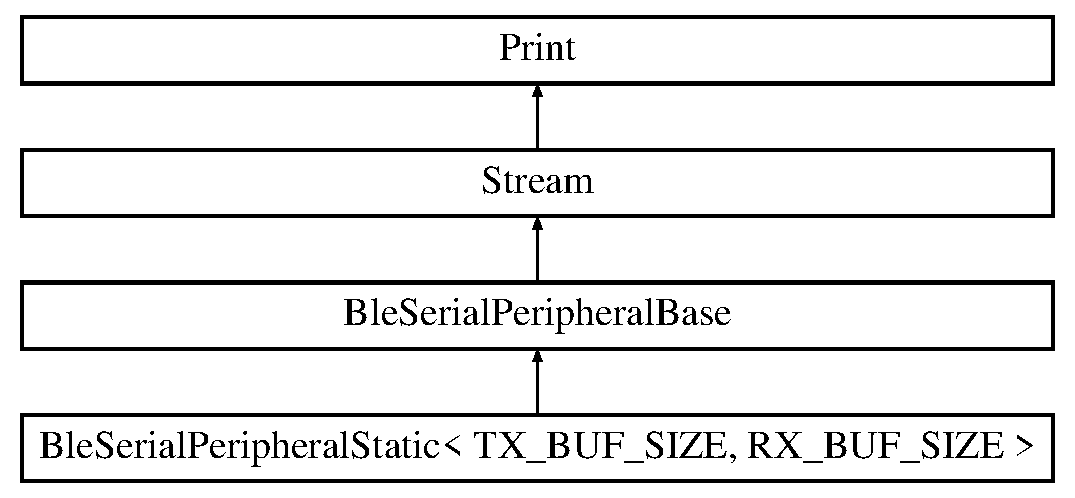
\includegraphics[height=4.000000cm]{class_ble_serial_peripheral_static}
\end{center}
\end{figure}
\subsection*{Additional Inherited Members}


\subsection{Detailed Description}
\subsubsection*{template$<$size\+\_\+t T\+X\+\_\+\+B\+U\+F\+\_\+\+S\+I\+ZE, size\+\_\+t R\+X\+\_\+\+B\+U\+F\+\_\+\+S\+I\+ZE$>$\newline
class Ble\+Serial\+Peripheral\+Static$<$ T\+X\+\_\+\+B\+U\+F\+\_\+\+S\+I\+Z\+E, R\+X\+\_\+\+B\+U\+F\+\_\+\+S\+I\+Z\+E $>$}

Ble\+Serial\+Peripheral with static buffers. This is the object you will normally create, as a global variable. 

T\+X\+\_\+\+B\+U\+F\+\_\+\+S\+I\+ZE is the size of the tx\+Buf in bytes. Since data is bunched up and sent out from loop this must be larger than the largest chunk of data you ever intend to send.

R\+X\+\_\+\+B\+U\+F\+\_\+\+S\+I\+ZE is the size of the rx\+Buf in bytes. Since data is received asynchronously, this must be larger than the most data you will receive and read in \mbox{\hyperlink{class_ble_serial_peripheral_base_a441dc005092891279967444cb2dc2ff2}{loop()}}.

You can only have one \mbox{\hyperlink{class_ble_serial_peripheral_static}{Ble\+Serial\+Peripheral\+Static}} or \mbox{\hyperlink{class_ble_serial_peripheral_base}{Ble\+Serial\+Peripheral\+Base}} object per device! 

The documentation for this class was generated from the following file\+:\begin{DoxyCompactItemize}
\item 
src/Ble\+Serial\+Peripheral\+R\+K.\+h\end{DoxyCompactItemize}

\hypertarget{class_print}{}\section{Print Class Reference}
\label{class_print}\index{Print@{Print}}


Class for printing to a stream or file.  




{\ttfamily \#include $<$spark\+\_\+wiring\+\_\+print.\+h$>$}

Inheritance diagram for Print\+:\begin{figure}[H]
\begin{center}
\leavevmode
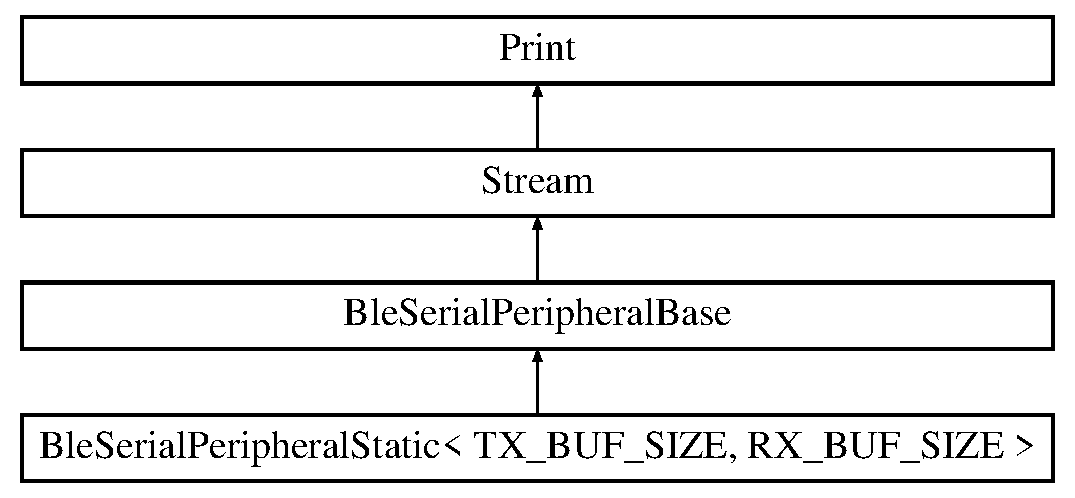
\includegraphics[height=4.000000cm]{class_print}
\end{center}
\end{figure}
\subsection*{Public Member Functions}
\begin{DoxyCompactItemize}
\item 
\mbox{\Hypertarget{class_print_a88a4a829fb5d589efb43955ad0cbddcc}\label{class_print_a88a4a829fb5d589efb43955ad0cbddcc}} 
int \mbox{\hyperlink{class_print_a88a4a829fb5d589efb43955ad0cbddcc}{get\+Write\+Error}} ()
\begin{DoxyCompactList}\small\item\em Return the last error code. 0 means no error. \end{DoxyCompactList}\item 
\mbox{\Hypertarget{class_print_aec9ecf84cc6d9087a650def3cefc459e}\label{class_print_aec9ecf84cc6d9087a650def3cefc459e}} 
void \mbox{\hyperlink{class_print_aec9ecf84cc6d9087a650def3cefc459e}{clear\+Write\+Error}} ()
\begin{DoxyCompactList}\small\item\em Clear the last error code to 0. \end{DoxyCompactList}\item 
virtual size\+\_\+t \mbox{\hyperlink{class_print_ab9195b97274029f693aaddce6c7a0021}{write}} (uint8\+\_\+t c)=0
\begin{DoxyCompactList}\small\item\em Write a single byte to the stream or file. \end{DoxyCompactList}\item 
size\+\_\+t \mbox{\hyperlink{class_print_a5b40e0e9cab1f2fe5bb0cb22ffe5adda}{write}} (const char $\ast$str)
\begin{DoxyCompactList}\small\item\em Write a null-\/terminated c-\/string the stream or file. \end{DoxyCompactList}\item 
virtual size\+\_\+t \mbox{\hyperlink{class_print_a88864e109589a5be9b0f5ba1327f8421}{write}} (const uint8\+\_\+t $\ast$buffer, size\+\_\+t size)
\begin{DoxyCompactList}\small\item\em Write a bytes specified by a buffer and length to the stream or file. \end{DoxyCompactList}\item 
\mbox{\Hypertarget{class_print_acfe80773011eb17dfb52c2fba517a093}\label{class_print_acfe80773011eb17dfb52c2fba517a093}} 
size\+\_\+t \mbox{\hyperlink{class_print_acfe80773011eb17dfb52c2fba517a093}{print}} (const char\mbox{[}$\,$\mbox{]})
\begin{DoxyCompactList}\small\item\em \mbox{\hyperlink{class_print}{Print}} a null-\/terminated array of char variables (a c-\/string) to the stream or file. \end{DoxyCompactList}\item 
\mbox{\Hypertarget{class_print_a1e411d07a8ffec5faf7ce485bac0f029}\label{class_print_a1e411d07a8ffec5faf7ce485bac0f029}} 
size\+\_\+t \mbox{\hyperlink{class_print_a1e411d07a8ffec5faf7ce485bac0f029}{print}} (char)
\begin{DoxyCompactList}\small\item\em \mbox{\hyperlink{class_print}{Print}} a single character to the stream or file. \end{DoxyCompactList}\item 
size\+\_\+t \mbox{\hyperlink{class_print_ae35481e77567618140cd58d8b96d3747}{print}} (unsigned char value, int base=D\+EC)
\begin{DoxyCompactList}\small\item\em \mbox{\hyperlink{class_print}{Print}} an unsigned char (byte value, 8 bits) in the specified base to the stream or file. \end{DoxyCompactList}\item 
size\+\_\+t \mbox{\hyperlink{class_print_aa28ddbde83b14df73b41c919ecc4478f}{print}} (int value, int base=D\+EC)
\begin{DoxyCompactList}\small\item\em \mbox{\hyperlink{class_print}{Print}} an int (32 bit integer) the specified base to the stream or file. \end{DoxyCompactList}\item 
size\+\_\+t \mbox{\hyperlink{class_print_afcd7d3a184df961a502643e4fb638c52}{print}} (unsigned int value, int base=D\+EC)
\begin{DoxyCompactList}\small\item\em \mbox{\hyperlink{class_print}{Print}} an unsigned int (32 bit unsigned integer) the specified base to the stream or file. \end{DoxyCompactList}\item 
size\+\_\+t \mbox{\hyperlink{class_print_a0c663ac015ebc037ea044ba2e2cf2947}{print}} (long value, int base=D\+EC)
\begin{DoxyCompactList}\small\item\em \mbox{\hyperlink{class_print}{Print}} a long (32 bit integer) the specified base to the stream or file. \end{DoxyCompactList}\item 
size\+\_\+t \mbox{\hyperlink{class_print_acb8c6dcd4339b024436002aa9a6f4be2}{print}} (unsigned long value, int base=D\+EC)
\begin{DoxyCompactList}\small\item\em \mbox{\hyperlink{class_print}{Print}} a unsigned long (32 bit unsigned integer) the specified base to the stream or file. \end{DoxyCompactList}\item 
size\+\_\+t \mbox{\hyperlink{class_print_ad89472bdb6539423a42d350beec02ff4}{print}} (double value, int dec=2)
\begin{DoxyCompactList}\small\item\em \mbox{\hyperlink{class_print}{Print}} a double floating point value to the stream or file. \end{DoxyCompactList}\item 
\mbox{\Hypertarget{class_print_a901b0f06ae34aab31b8fbb4298f0596e}\label{class_print_a901b0f06ae34aab31b8fbb4298f0596e}} 
size\+\_\+t \mbox{\hyperlink{class_print_a901b0f06ae34aab31b8fbb4298f0596e}{print}} (const Printable \&)
\begin{DoxyCompactList}\small\item\em \mbox{\hyperlink{class_print}{Print}} an object derived from Printable to the stream or file. \end{DoxyCompactList}\item 
\mbox{\Hypertarget{class_print_ad337ce3f7977411b7d34d47a51e5737e}\label{class_print_ad337ce3f7977411b7d34d47a51e5737e}} 
size\+\_\+t \mbox{\hyperlink{class_print_ad337ce3f7977411b7d34d47a51e5737e}{println}} (const char\mbox{[}$\,$\mbox{]})
\begin{DoxyCompactList}\small\item\em \mbox{\hyperlink{class_print}{Print}} a null-\/terminated array of char variables (a c-\/string) plus a C\+R\+LF end-\/of-\/line terminator to the stream or file. \end{DoxyCompactList}\item 
\mbox{\Hypertarget{class_print_a80fdd92db4b396062586bcb3e08d3835}\label{class_print_a80fdd92db4b396062586bcb3e08d3835}} 
size\+\_\+t \mbox{\hyperlink{class_print_a80fdd92db4b396062586bcb3e08d3835}{println}} (char value)
\begin{DoxyCompactList}\small\item\em \mbox{\hyperlink{class_print}{Print}} a single character plus a C\+R\+LF end-\/of-\/line terminator to the stream or file. \end{DoxyCompactList}\item 
size\+\_\+t \mbox{\hyperlink{class_print_a000b3fd5b723cb6c7db0d3231a9ef2f8}{println}} (unsigned char value, int base=D\+EC)
\begin{DoxyCompactList}\small\item\em \mbox{\hyperlink{class_print}{Print}} an unsigned char (byte value. 8 bits) in the specified base plus a C\+R\+LF end-\/of-\/line terminator to the stream or file. \end{DoxyCompactList}\item 
size\+\_\+t \mbox{\hyperlink{class_print_a82aa91bbd859f28a0a3b4869e5bfcadd}{println}} (int value, int base=D\+EC)
\begin{DoxyCompactList}\small\item\em \mbox{\hyperlink{class_print}{Print}} an int (32 bit integer) the specified base to plus a C\+R\+LF end-\/of-\/line terminator the stream or file. \end{DoxyCompactList}\item 
size\+\_\+t \mbox{\hyperlink{class_print_a2608232c1f10f654111ff447de16d60b}{println}} (unsigned int value, int base=D\+EC)
\begin{DoxyCompactList}\small\item\em \mbox{\hyperlink{class_print}{Print}} an unsigned int (32 bit unsigned integer) the specified base plus a C\+R\+LF end-\/of-\/line terminator to the stream or file. \end{DoxyCompactList}\item 
size\+\_\+t \mbox{\hyperlink{class_print_a82bbe59b28440c29e55ff3597eb45376}{println}} (long value, int base=D\+EC)
\begin{DoxyCompactList}\small\item\em \mbox{\hyperlink{class_print}{Print}} a long (32 bit signed integer) the specified base plus a C\+R\+LF end-\/of-\/line terminator to the stream or file. \end{DoxyCompactList}\item 
size\+\_\+t \mbox{\hyperlink{class_print_afa936d7e8dd329d9162f2cd28f42681e}{println}} (unsigned long value, int base=D\+EC)
\begin{DoxyCompactList}\small\item\em \mbox{\hyperlink{class_print}{Print}} a unsigned long (32 bit unsigned integer) the specified base plus a C\+R\+LF end-\/of-\/line terminator to the stream or file. \end{DoxyCompactList}\item 
size\+\_\+t \mbox{\hyperlink{class_print_a178b90baf9f74f0945f5c64aafec59ea}{println}} (double value, int dec=2)
\begin{DoxyCompactList}\small\item\em \mbox{\hyperlink{class_print}{Print}} a double floating point value plus a C\+R\+LF end-\/of-\/line terminator to the stream or file. \end{DoxyCompactList}\item 
\mbox{\Hypertarget{class_print_a20f9e104153b62e720c9b4c348b44f00}\label{class_print_a20f9e104153b62e720c9b4c348b44f00}} 
size\+\_\+t \mbox{\hyperlink{class_print_a20f9e104153b62e720c9b4c348b44f00}{println}} (const Printable \&)
\begin{DoxyCompactList}\small\item\em \mbox{\hyperlink{class_print}{Print}} an object derived from Printable plus a C\+R\+LF end-\/of-\/line terminator to the stream or file. \end{DoxyCompactList}\item 
\mbox{\Hypertarget{class_print_a169b128f9e22f0c15883768f580541a2}\label{class_print_a169b128f9e22f0c15883768f580541a2}} 
size\+\_\+t \mbox{\hyperlink{class_print_a169b128f9e22f0c15883768f580541a2}{println}} (void)
\begin{DoxyCompactList}\small\item\em \mbox{\hyperlink{class_print}{Print}} a C\+R\+LF end-\/of-\/line terminator to the stream or file. \end{DoxyCompactList}\item 
{\footnotesize template$<$typename... Args$>$ }\\size\+\_\+t \mbox{\hyperlink{class_print_a08a461c9fee5fd8f5795d6e9f61e3d5b}{printf}} (const char $\ast$format, Args... args)
\begin{DoxyCompactList}\small\item\em \mbox{\hyperlink{class_print}{Print}} using printf-\/style formatting to the stream or file. \end{DoxyCompactList}\item 
{\footnotesize template$<$typename... Args$>$ }\\size\+\_\+t \mbox{\hyperlink{class_print_afa41aa5211c54b7b4d79b9286880c337}{printlnf}} (const char $\ast$format, Args... args)
\begin{DoxyCompactList}\small\item\em \mbox{\hyperlink{class_print}{Print}} using printf-\/style formatting plus a C\+R\+LF end-\/of-\/line terminator to the stream or file. \end{DoxyCompactList}\end{DoxyCompactItemize}


\subsection{Detailed Description}
Class for printing to a stream or file. 

Various classes include serial, T\+CP network streams, and files inherit from this and can use these methods. 

\subsection{Member Function Documentation}
\mbox{\Hypertarget{class_print_ae35481e77567618140cd58d8b96d3747}\label{class_print_ae35481e77567618140cd58d8b96d3747}} 
\index{Print@{Print}!print@{print}}
\index{print@{print}!Print@{Print}}
\subsubsection{\texorpdfstring{print()}{print()}\hspace{0.1cm}{\footnotesize\ttfamily [1/6]}}
{\footnotesize\ttfamily size\+\_\+t Print\+::print (\begin{DoxyParamCaption}\item[{unsigned char}]{value,  }\item[{int}]{base = {\ttfamily DEC} }\end{DoxyParamCaption})}



\mbox{\hyperlink{class_print}{Print}} an unsigned char (byte value, 8 bits) in the specified base to the stream or file. 


\begin{DoxyParams}{Parameters}
{\em value} & The value to print. \\
\hline
{\em base} & The base to print. Default is D\+EC (decimal). Other values are H\+EX (hexadecimal), O\+CT (octal), and B\+IN (binary). \\
\hline
\end{DoxyParams}
\mbox{\Hypertarget{class_print_aa28ddbde83b14df73b41c919ecc4478f}\label{class_print_aa28ddbde83b14df73b41c919ecc4478f}} 
\index{Print@{Print}!print@{print}}
\index{print@{print}!Print@{Print}}
\subsubsection{\texorpdfstring{print()}{print()}\hspace{0.1cm}{\footnotesize\ttfamily [2/6]}}
{\footnotesize\ttfamily size\+\_\+t Print\+::print (\begin{DoxyParamCaption}\item[{int}]{value,  }\item[{int}]{base = {\ttfamily DEC} }\end{DoxyParamCaption})}



\mbox{\hyperlink{class_print}{Print}} an int (32 bit integer) the specified base to the stream or file. 


\begin{DoxyParams}{Parameters}
{\em value} & The value to print. \\
\hline
{\em base} & The base to print. Default is D\+EC (decimal). Other values are H\+EX (hexadecimal), O\+CT (octal), and B\+IN (binary). \\
\hline
\end{DoxyParams}
\mbox{\Hypertarget{class_print_afcd7d3a184df961a502643e4fb638c52}\label{class_print_afcd7d3a184df961a502643e4fb638c52}} 
\index{Print@{Print}!print@{print}}
\index{print@{print}!Print@{Print}}
\subsubsection{\texorpdfstring{print()}{print()}\hspace{0.1cm}{\footnotesize\ttfamily [3/6]}}
{\footnotesize\ttfamily size\+\_\+t Print\+::print (\begin{DoxyParamCaption}\item[{unsigned int}]{value,  }\item[{int}]{base = {\ttfamily DEC} }\end{DoxyParamCaption})}



\mbox{\hyperlink{class_print}{Print}} an unsigned int (32 bit unsigned integer) the specified base to the stream or file. 


\begin{DoxyParams}{Parameters}
{\em value} & The value to print. \\
\hline
{\em base} & The base to print. Default is D\+EC (decimal). Other values are H\+EX (hexadecimal), O\+CT (octal), and B\+IN (binary). \\
\hline
\end{DoxyParams}
\mbox{\Hypertarget{class_print_a0c663ac015ebc037ea044ba2e2cf2947}\label{class_print_a0c663ac015ebc037ea044ba2e2cf2947}} 
\index{Print@{Print}!print@{print}}
\index{print@{print}!Print@{Print}}
\subsubsection{\texorpdfstring{print()}{print()}\hspace{0.1cm}{\footnotesize\ttfamily [4/6]}}
{\footnotesize\ttfamily size\+\_\+t Print\+::print (\begin{DoxyParamCaption}\item[{long}]{value,  }\item[{int}]{base = {\ttfamily DEC} }\end{DoxyParamCaption})}



\mbox{\hyperlink{class_print}{Print}} a long (32 bit integer) the specified base to the stream or file. 


\begin{DoxyParams}{Parameters}
{\em value} & The value to print. \\
\hline
{\em base} & The base to print. Default is D\+EC (decimal). Other values are H\+EX (hexadecimal), O\+CT (octal), and B\+IN (binary). \\
\hline
\end{DoxyParams}
\mbox{\Hypertarget{class_print_acb8c6dcd4339b024436002aa9a6f4be2}\label{class_print_acb8c6dcd4339b024436002aa9a6f4be2}} 
\index{Print@{Print}!print@{print}}
\index{print@{print}!Print@{Print}}
\subsubsection{\texorpdfstring{print()}{print()}\hspace{0.1cm}{\footnotesize\ttfamily [5/6]}}
{\footnotesize\ttfamily size\+\_\+t Print\+::print (\begin{DoxyParamCaption}\item[{unsigned long}]{value,  }\item[{int}]{base = {\ttfamily DEC} }\end{DoxyParamCaption})}



\mbox{\hyperlink{class_print}{Print}} a unsigned long (32 bit unsigned integer) the specified base to the stream or file. 


\begin{DoxyParams}{Parameters}
{\em value} & The value to print. \\
\hline
{\em base} & The base to print. Default is D\+EC (decimal). Other values are H\+EX (hexadecimal), O\+CT (octal), and B\+IN (binary). \\
\hline
\end{DoxyParams}
\mbox{\Hypertarget{class_print_ad89472bdb6539423a42d350beec02ff4}\label{class_print_ad89472bdb6539423a42d350beec02ff4}} 
\index{Print@{Print}!print@{print}}
\index{print@{print}!Print@{Print}}
\subsubsection{\texorpdfstring{print()}{print()}\hspace{0.1cm}{\footnotesize\ttfamily [6/6]}}
{\footnotesize\ttfamily size\+\_\+t Print\+::print (\begin{DoxyParamCaption}\item[{double}]{value,  }\item[{int}]{dec = {\ttfamily 2} }\end{DoxyParamCaption})}



\mbox{\hyperlink{class_print}{Print}} a double floating point value to the stream or file. 


\begin{DoxyParams}{Parameters}
{\em value} & The value to print. \\
\hline
{\em dec} & The number of decimal places to include for the fractional part. Default\+: 2 \\
\hline
\end{DoxyParams}
\mbox{\Hypertarget{class_print_a08a461c9fee5fd8f5795d6e9f61e3d5b}\label{class_print_a08a461c9fee5fd8f5795d6e9f61e3d5b}} 
\index{Print@{Print}!printf@{printf}}
\index{printf@{printf}!Print@{Print}}
\subsubsection{\texorpdfstring{printf()}{printf()}}
{\footnotesize\ttfamily template$<$typename... Args$>$ \\
size\+\_\+t Print\+::printf (\begin{DoxyParamCaption}\item[{const char $\ast$}]{format,  }\item[{Args...}]{args }\end{DoxyParamCaption})\hspace{0.3cm}{\ttfamily [inline]}}



\mbox{\hyperlink{class_print}{Print}} using printf-\/style formatting to the stream or file. 


\begin{DoxyParams}{Parameters}
{\em format} & printf-\/style formatting string\\
\hline
{\em args} & variable arguments \\
\hline
\end{DoxyParams}
\mbox{\Hypertarget{class_print_a000b3fd5b723cb6c7db0d3231a9ef2f8}\label{class_print_a000b3fd5b723cb6c7db0d3231a9ef2f8}} 
\index{Print@{Print}!println@{println}}
\index{println@{println}!Print@{Print}}
\subsubsection{\texorpdfstring{println()}{println()}\hspace{0.1cm}{\footnotesize\ttfamily [1/6]}}
{\footnotesize\ttfamily size\+\_\+t Print\+::println (\begin{DoxyParamCaption}\item[{unsigned char}]{value,  }\item[{int}]{base = {\ttfamily DEC} }\end{DoxyParamCaption})}



\mbox{\hyperlink{class_print}{Print}} an unsigned char (byte value. 8 bits) in the specified base plus a C\+R\+LF end-\/of-\/line terminator to the stream or file. 


\begin{DoxyParams}{Parameters}
{\em value} & The value to print. \\
\hline
{\em base} & The base to print. Default is D\+EC (decimal). Other values are H\+EX (hexadecimal), O\+CT (octal), and B\+IN (binary). \\
\hline
\end{DoxyParams}
\mbox{\Hypertarget{class_print_a82aa91bbd859f28a0a3b4869e5bfcadd}\label{class_print_a82aa91bbd859f28a0a3b4869e5bfcadd}} 
\index{Print@{Print}!println@{println}}
\index{println@{println}!Print@{Print}}
\subsubsection{\texorpdfstring{println()}{println()}\hspace{0.1cm}{\footnotesize\ttfamily [2/6]}}
{\footnotesize\ttfamily size\+\_\+t Print\+::println (\begin{DoxyParamCaption}\item[{int}]{value,  }\item[{int}]{base = {\ttfamily DEC} }\end{DoxyParamCaption})}



\mbox{\hyperlink{class_print}{Print}} an int (32 bit integer) the specified base to plus a C\+R\+LF end-\/of-\/line terminator the stream or file. 


\begin{DoxyParams}{Parameters}
{\em value} & The value to print \\
\hline
{\em base} & The base to print. Default is D\+EC (decimal). Other values are H\+EX (hexadecimal), O\+CT (octal), and B\+IN (binary). \\
\hline
\end{DoxyParams}
\mbox{\Hypertarget{class_print_a2608232c1f10f654111ff447de16d60b}\label{class_print_a2608232c1f10f654111ff447de16d60b}} 
\index{Print@{Print}!println@{println}}
\index{println@{println}!Print@{Print}}
\subsubsection{\texorpdfstring{println()}{println()}\hspace{0.1cm}{\footnotesize\ttfamily [3/6]}}
{\footnotesize\ttfamily size\+\_\+t Print\+::println (\begin{DoxyParamCaption}\item[{unsigned int}]{value,  }\item[{int}]{base = {\ttfamily DEC} }\end{DoxyParamCaption})}



\mbox{\hyperlink{class_print}{Print}} an unsigned int (32 bit unsigned integer) the specified base plus a C\+R\+LF end-\/of-\/line terminator to the stream or file. 


\begin{DoxyParams}{Parameters}
{\em value} & The value to print \\
\hline
{\em base} & The base to print. Default is D\+EC (decimal). Other values are H\+EX (hexadecimal), O\+CT (octal), and B\+IN (binary). \\
\hline
\end{DoxyParams}
\mbox{\Hypertarget{class_print_a82bbe59b28440c29e55ff3597eb45376}\label{class_print_a82bbe59b28440c29e55ff3597eb45376}} 
\index{Print@{Print}!println@{println}}
\index{println@{println}!Print@{Print}}
\subsubsection{\texorpdfstring{println()}{println()}\hspace{0.1cm}{\footnotesize\ttfamily [4/6]}}
{\footnotesize\ttfamily size\+\_\+t Print\+::println (\begin{DoxyParamCaption}\item[{long}]{value,  }\item[{int}]{base = {\ttfamily DEC} }\end{DoxyParamCaption})}



\mbox{\hyperlink{class_print}{Print}} a long (32 bit signed integer) the specified base plus a C\+R\+LF end-\/of-\/line terminator to the stream or file. 


\begin{DoxyParams}{Parameters}
{\em value} & The value to print \\
\hline
{\em base} & The base to print. Default is D\+EC (decimal). Other values are H\+EX (hexadecimal), O\+CT (octal), and B\+IN (binary). \\
\hline
\end{DoxyParams}
\mbox{\Hypertarget{class_print_afa936d7e8dd329d9162f2cd28f42681e}\label{class_print_afa936d7e8dd329d9162f2cd28f42681e}} 
\index{Print@{Print}!println@{println}}
\index{println@{println}!Print@{Print}}
\subsubsection{\texorpdfstring{println()}{println()}\hspace{0.1cm}{\footnotesize\ttfamily [5/6]}}
{\footnotesize\ttfamily size\+\_\+t Print\+::println (\begin{DoxyParamCaption}\item[{unsigned long}]{value,  }\item[{int}]{base = {\ttfamily DEC} }\end{DoxyParamCaption})}



\mbox{\hyperlink{class_print}{Print}} a unsigned long (32 bit unsigned integer) the specified base plus a C\+R\+LF end-\/of-\/line terminator to the stream or file. 


\begin{DoxyParams}{Parameters}
{\em value} & The value to print. \\
\hline
{\em base} & The base to print. Default is D\+EC (decimal). Other values are H\+EX (hexadecimal), O\+CT (octal), and B\+IN (binary). \\
\hline
\end{DoxyParams}
\mbox{\Hypertarget{class_print_a178b90baf9f74f0945f5c64aafec59ea}\label{class_print_a178b90baf9f74f0945f5c64aafec59ea}} 
\index{Print@{Print}!println@{println}}
\index{println@{println}!Print@{Print}}
\subsubsection{\texorpdfstring{println()}{println()}\hspace{0.1cm}{\footnotesize\ttfamily [6/6]}}
{\footnotesize\ttfamily size\+\_\+t Print\+::println (\begin{DoxyParamCaption}\item[{double}]{value,  }\item[{int}]{dec = {\ttfamily 2} }\end{DoxyParamCaption})}



\mbox{\hyperlink{class_print}{Print}} a double floating point value plus a C\+R\+LF end-\/of-\/line terminator to the stream or file. 


\begin{DoxyParams}{Parameters}
{\em value} & The value to print. \\
\hline
{\em dec} & The number of decimal places to include for the fractional part. Default\+: 2 \\
\hline
\end{DoxyParams}
\mbox{\Hypertarget{class_print_afa41aa5211c54b7b4d79b9286880c337}\label{class_print_afa41aa5211c54b7b4d79b9286880c337}} 
\index{Print@{Print}!printlnf@{printlnf}}
\index{printlnf@{printlnf}!Print@{Print}}
\subsubsection{\texorpdfstring{printlnf()}{printlnf()}}
{\footnotesize\ttfamily template$<$typename... Args$>$ \\
size\+\_\+t Print\+::printlnf (\begin{DoxyParamCaption}\item[{const char $\ast$}]{format,  }\item[{Args...}]{args }\end{DoxyParamCaption})\hspace{0.3cm}{\ttfamily [inline]}}



\mbox{\hyperlink{class_print}{Print}} using printf-\/style formatting plus a C\+R\+LF end-\/of-\/line terminator to the stream or file. 


\begin{DoxyParams}{Parameters}
{\em format} & printf-\/style formatting string\\
\hline
{\em args} & variable arguments \\
\hline
\end{DoxyParams}
\mbox{\Hypertarget{class_print_ab9195b97274029f693aaddce6c7a0021}\label{class_print_ab9195b97274029f693aaddce6c7a0021}} 
\index{Print@{Print}!write@{write}}
\index{write@{write}!Print@{Print}}
\subsubsection{\texorpdfstring{write()}{write()}\hspace{0.1cm}{\footnotesize\ttfamily [1/3]}}
{\footnotesize\ttfamily virtual size\+\_\+t Print\+::write (\begin{DoxyParamCaption}\item[{uint8\+\_\+t}]{c }\end{DoxyParamCaption})\hspace{0.3cm}{\ttfamily [pure virtual]}}



Write a single byte to the stream or file. 


\begin{DoxyParams}{Parameters}
{\em c} & The byte to write. All values 0 -\/ 255 are allowed. \\
\hline
\end{DoxyParams}


Implemented in \mbox{\hyperlink{class_ble_serial_peripheral_base_ac041322685f26d921f60d01a2ed99e83}{Ble\+Serial\+Peripheral\+Base}}.

\mbox{\Hypertarget{class_print_a5b40e0e9cab1f2fe5bb0cb22ffe5adda}\label{class_print_a5b40e0e9cab1f2fe5bb0cb22ffe5adda}} 
\index{Print@{Print}!write@{write}}
\index{write@{write}!Print@{Print}}
\subsubsection{\texorpdfstring{write()}{write()}\hspace{0.1cm}{\footnotesize\ttfamily [2/3]}}
{\footnotesize\ttfamily size\+\_\+t Print\+::write (\begin{DoxyParamCaption}\item[{const char $\ast$}]{str }\end{DoxyParamCaption})\hspace{0.3cm}{\ttfamily [inline]}}



Write a null-\/terminated c-\/string the stream or file. 


\begin{DoxyParams}{Parameters}
{\em str} & point to a null-\/terminated c-\/string. \\
\hline
\end{DoxyParams}
\mbox{\Hypertarget{class_print_a88864e109589a5be9b0f5ba1327f8421}\label{class_print_a88864e109589a5be9b0f5ba1327f8421}} 
\index{Print@{Print}!write@{write}}
\index{write@{write}!Print@{Print}}
\subsubsection{\texorpdfstring{write()}{write()}\hspace{0.1cm}{\footnotesize\ttfamily [3/3]}}
{\footnotesize\ttfamily virtual size\+\_\+t Print\+::write (\begin{DoxyParamCaption}\item[{const uint8\+\_\+t $\ast$}]{buffer,  }\item[{size\+\_\+t}]{size }\end{DoxyParamCaption})\hspace{0.3cm}{\ttfamily [virtual]}}



Write a bytes specified by a buffer and length to the stream or file. 


\begin{DoxyParams}{Parameters}
{\em buffer} & pointer to the buffer. The data does not need to be null-\/terminated. \\
\hline
{\em size} & size in bytes \\
\hline
\end{DoxyParams}


The documentation for this class was generated from the following file\+:\begin{DoxyCompactItemize}
\item 
docs/src/\mbox{\hyperlink{spark__wiring__print_8h}{spark\+\_\+wiring\+\_\+print.\+h}}\end{DoxyCompactItemize}

\hypertarget{class_ring_buffer}{}\section{Ring\+Buffer$<$ T $>$ Class Template Reference}
\label{class_ring_buffer}\index{Ring\+Buffer$<$ T $>$@{Ring\+Buffer$<$ T $>$}}


Thread and interrupt-\/safe (with caveats) circular buffer (ring buffer) class.  




{\ttfamily \#include $<$Ring\+Buffer.\+h$>$}

\subsection*{Public Member Functions}
\begin{DoxyCompactItemize}
\item 
\mbox{\hyperlink{class_ring_buffer_a234232078f579680a091bc504b5eee5e}{Ring\+Buffer}} (T $\ast$elems, size\+\_\+t size)
\begin{DoxyCompactList}\small\item\em Construct a buffer of size elements of T. \end{DoxyCompactList}\item 
\mbox{\Hypertarget{class_ring_buffer_a2ea502f6493ca669f07f9f01a4a94bdb}\label{class_ring_buffer_a2ea502f6493ca669f07f9f01a4a94bdb}} 
\mbox{\hyperlink{class_ring_buffer_a2ea502f6493ca669f07f9f01a4a94bdb}{$\sim$\+Ring\+Buffer}} ()
\begin{DoxyCompactList}\small\item\em Destructor. \end{DoxyCompactList}\item 
size\+\_\+t \mbox{\hyperlink{class_ring_buffer_a2d77169348cd228b343ba2245e1ce371}{available\+For\+Read}} () const
\begin{DoxyCompactList}\small\item\em Returns the number of elements that can be read right now (0 = nothing can be read right now) \end{DoxyCompactList}\item 
T $\ast$ \mbox{\hyperlink{class_ring_buffer_a724ce39b381489539fda406e06596a1d}{pre\+Read}} () const
\begin{DoxyCompactList}\small\item\em Non-\/copy version of read. Returns a pointer to the data to be read next or N\+U\+LL if there is no data right now. \end{DoxyCompactList}\item 
void \mbox{\hyperlink{class_ring_buffer_aad9eebd3dc4cc774666467de89c6de86}{post\+Read}} ()
\begin{DoxyCompactList}\small\item\em Indicates that you have finished reading the data in the pointer returned by \mbox{\hyperlink{class_ring_buffer_a724ce39b381489539fda406e06596a1d}{pre\+Read()}} and it can be reused. \end{DoxyCompactList}\item 
bool \mbox{\hyperlink{class_ring_buffer_af4ab31038d40a4075f4f23b7f2c970cd}{read}} (T $\ast$elem)
\begin{DoxyCompactList}\small\item\em Read with copy. You can use this instead of \mbox{\hyperlink{class_ring_buffer_a724ce39b381489539fda406e06596a1d}{pre\+Read()}} and \mbox{\hyperlink{class_ring_buffer_aad9eebd3dc4cc774666467de89c6de86}{post\+Read()}}. \end{DoxyCompactList}\item 
\mbox{\Hypertarget{class_ring_buffer_a5f17853814de662a9f15a14fddfea4bf}\label{class_ring_buffer_a5f17853814de662a9f15a14fddfea4bf}} 
void \mbox{\hyperlink{class_ring_buffer_a5f17853814de662a9f15a14fddfea4bf}{read\+Clear}} ()
\begin{DoxyCompactList}\small\item\em Clear outstanding entries, called from the read thread. \end{DoxyCompactList}\item 
T $\ast$ \mbox{\hyperlink{class_ring_buffer_a60177190baecb3c438f8392d6f9a35f7}{pre\+Write}} () const
\begin{DoxyCompactList}\small\item\em Non-\/copy version of write. Returns a pointer to the buffer to write to or N\+U\+LL if there is no space. \end{DoxyCompactList}\item 
\mbox{\Hypertarget{class_ring_buffer_a7d2e2f6098053c51451ff2bd35fa2252}\label{class_ring_buffer_a7d2e2f6098053c51451ff2bd35fa2252}} 
void \mbox{\hyperlink{class_ring_buffer_a7d2e2f6098053c51451ff2bd35fa2252}{post\+Write}} ()
\begin{DoxyCompactList}\small\item\em Commits the write. Only call if \mbox{\hyperlink{class_ring_buffer_a60177190baecb3c438f8392d6f9a35f7}{pre\+Write()}} returned a non-\/\+N\+U\+LL value. \end{DoxyCompactList}\item 
bool \mbox{\hyperlink{class_ring_buffer_a1a9e393325923ed035b16a5b067a3951}{write}} (const T $\ast$elem)
\begin{DoxyCompactList}\small\item\em Write with copy. You can use this instead of \mbox{\hyperlink{class_ring_buffer_a60177190baecb3c438f8392d6f9a35f7}{pre\+Write()}} and \mbox{\hyperlink{class_ring_buffer_a7d2e2f6098053c51451ff2bd35fa2252}{post\+Write()}}. elem is copied. \end{DoxyCompactList}\end{DoxyCompactItemize}


\subsection{Detailed Description}
\subsubsection*{template$<$class T$>$\newline
class Ring\+Buffer$<$ T $>$}

Thread and interrupt-\/safe (with caveats) circular buffer (ring buffer) class. 

Home\+: \href{https://github.com/rickkas7/SerialBufferRK}{\tt https\+://github.\+com/rickkas7/\+Serial\+Buffer\+RK} License\+: M\+IT This class assumes a single reader thread and a single writer thread (or interrupt). For example, it works great if you read out of loop() and write from a single interrupt handler. It is not safe for multiple reader or multiple writer use cases!

Assumption\+: Writing a size\+\_\+t value is atomic. It definitely is safe on A\+RM processors. 

\subsection{Constructor \& Destructor Documentation}
\mbox{\Hypertarget{class_ring_buffer_a234232078f579680a091bc504b5eee5e}\label{class_ring_buffer_a234232078f579680a091bc504b5eee5e}} 
\index{Ring\+Buffer@{Ring\+Buffer}!Ring\+Buffer@{Ring\+Buffer}}
\index{Ring\+Buffer@{Ring\+Buffer}!Ring\+Buffer@{Ring\+Buffer}}
\subsubsection{\texorpdfstring{Ring\+Buffer()}{RingBuffer()}}
{\footnotesize\ttfamily template$<$class T$>$ \\
\mbox{\hyperlink{class_ring_buffer}{Ring\+Buffer}}$<$ T $>$\+::\mbox{\hyperlink{class_ring_buffer}{Ring\+Buffer}} (\begin{DoxyParamCaption}\item[{T $\ast$}]{elems,  }\item[{size\+\_\+t}]{size }\end{DoxyParamCaption})\hspace{0.3cm}{\ttfamily [inline]}}



Construct a buffer of size elements of T. 


\begin{DoxyParams}{Parameters}
{\em elems} & Pointer to a buffer of size elements of type T\\
\hline
{\em size} & Number of elements \\
\hline
\end{DoxyParams}


\subsection{Member Function Documentation}
\mbox{\Hypertarget{class_ring_buffer_a2d77169348cd228b343ba2245e1ce371}\label{class_ring_buffer_a2d77169348cd228b343ba2245e1ce371}} 
\index{Ring\+Buffer@{Ring\+Buffer}!available\+For\+Read@{available\+For\+Read}}
\index{available\+For\+Read@{available\+For\+Read}!Ring\+Buffer@{Ring\+Buffer}}
\subsubsection{\texorpdfstring{available\+For\+Read()}{availableForRead()}}
{\footnotesize\ttfamily template$<$class T$>$ \\
size\+\_\+t \mbox{\hyperlink{class_ring_buffer}{Ring\+Buffer}}$<$ T $>$\+::available\+For\+Read (\begin{DoxyParamCaption}{ }\end{DoxyParamCaption}) const\hspace{0.3cm}{\ttfamily [inline]}}



Returns the number of elements that can be read right now (0 = nothing can be read right now) 

This is mainly for informational purposes. It\textquotesingle{}s more efficient to call \mbox{\hyperlink{class_ring_buffer_a724ce39b381489539fda406e06596a1d}{pre\+Read()}} and check for a non-\/\+N\+U\+LL return value than it is to call \mbox{\hyperlink{class_ring_buffer_a2d77169348cd228b343ba2245e1ce371}{available\+For\+Read()}}. \mbox{\Hypertarget{class_ring_buffer_aad9eebd3dc4cc774666467de89c6de86}\label{class_ring_buffer_aad9eebd3dc4cc774666467de89c6de86}} 
\index{Ring\+Buffer@{Ring\+Buffer}!post\+Read@{post\+Read}}
\index{post\+Read@{post\+Read}!Ring\+Buffer@{Ring\+Buffer}}
\subsubsection{\texorpdfstring{post\+Read()}{postRead()}}
{\footnotesize\ttfamily template$<$class T$>$ \\
void \mbox{\hyperlink{class_ring_buffer}{Ring\+Buffer}}$<$ T $>$\+::post\+Read (\begin{DoxyParamCaption}{ }\end{DoxyParamCaption})\hspace{0.3cm}{\ttfamily [inline]}}



Indicates that you have finished reading the data in the pointer returned by \mbox{\hyperlink{class_ring_buffer_a724ce39b381489539fda406e06596a1d}{pre\+Read()}} and it can be reused. 

Only call \mbox{\hyperlink{class_ring_buffer_aad9eebd3dc4cc774666467de89c6de86}{post\+Read()}} if \mbox{\hyperlink{class_ring_buffer_a724ce39b381489539fda406e06596a1d}{pre\+Read()}} returned a non-\/null value! \mbox{\Hypertarget{class_ring_buffer_a724ce39b381489539fda406e06596a1d}\label{class_ring_buffer_a724ce39b381489539fda406e06596a1d}} 
\index{Ring\+Buffer@{Ring\+Buffer}!pre\+Read@{pre\+Read}}
\index{pre\+Read@{pre\+Read}!Ring\+Buffer@{Ring\+Buffer}}
\subsubsection{\texorpdfstring{pre\+Read()}{preRead()}}
{\footnotesize\ttfamily template$<$class T$>$ \\
T$\ast$ \mbox{\hyperlink{class_ring_buffer}{Ring\+Buffer}}$<$ T $>$\+::pre\+Read (\begin{DoxyParamCaption}{ }\end{DoxyParamCaption}) const\hspace{0.3cm}{\ttfamily [inline]}}



Non-\/copy version of read. Returns a pointer to the data to be read next or N\+U\+LL if there is no data right now. 

If \mbox{\hyperlink{class_ring_buffer_a724ce39b381489539fda406e06596a1d}{pre\+Read()}} returns a non-\/null value you must call \mbox{\hyperlink{class_ring_buffer_aad9eebd3dc4cc774666467de89c6de86}{post\+Read()}} to consume the data, otherwise the next time you call \mbox{\hyperlink{class_ring_buffer_a724ce39b381489539fda406e06596a1d}{pre\+Read()}} you\textquotesingle{}ll get the same data back. Don\textquotesingle{}t call \mbox{\hyperlink{class_ring_buffer_aad9eebd3dc4cc774666467de89c6de86}{post\+Read()}} if you get N\+U\+LL back from \mbox{\hyperlink{class_ring_buffer_a724ce39b381489539fda406e06596a1d}{pre\+Read()}}!

It\textquotesingle{}s OK to not call \mbox{\hyperlink{class_ring_buffer_aad9eebd3dc4cc774666467de89c6de86}{post\+Read()}} if you\textquotesingle{}re doing a peek at the data -\/ look at the data that will be read without removing it. \mbox{\Hypertarget{class_ring_buffer_a60177190baecb3c438f8392d6f9a35f7}\label{class_ring_buffer_a60177190baecb3c438f8392d6f9a35f7}} 
\index{Ring\+Buffer@{Ring\+Buffer}!pre\+Write@{pre\+Write}}
\index{pre\+Write@{pre\+Write}!Ring\+Buffer@{Ring\+Buffer}}
\subsubsection{\texorpdfstring{pre\+Write()}{preWrite()}}
{\footnotesize\ttfamily template$<$class T$>$ \\
T$\ast$ \mbox{\hyperlink{class_ring_buffer}{Ring\+Buffer}}$<$ T $>$\+::pre\+Write (\begin{DoxyParamCaption}{ }\end{DoxyParamCaption}) const\hspace{0.3cm}{\ttfamily [inline]}}



Non-\/copy version of write. Returns a pointer to the buffer to write to or N\+U\+LL if there is no space. 

If \mbox{\hyperlink{class_ring_buffer_a60177190baecb3c438f8392d6f9a35f7}{pre\+Write()}} returns a non-\/null value you must call \mbox{\hyperlink{class_ring_buffer_a7d2e2f6098053c51451ff2bd35fa2252}{post\+Write()}} to commit the data, otherwise the data will not be saved. Don\textquotesingle{}t call \mbox{\hyperlink{class_ring_buffer_a7d2e2f6098053c51451ff2bd35fa2252}{post\+Write()}} if you get N\+U\+LL back from \mbox{\hyperlink{class_ring_buffer_a60177190baecb3c438f8392d6f9a35f7}{pre\+Write()}}! \mbox{\Hypertarget{class_ring_buffer_af4ab31038d40a4075f4f23b7f2c970cd}\label{class_ring_buffer_af4ab31038d40a4075f4f23b7f2c970cd}} 
\index{Ring\+Buffer@{Ring\+Buffer}!read@{read}}
\index{read@{read}!Ring\+Buffer@{Ring\+Buffer}}
\subsubsection{\texorpdfstring{read()}{read()}}
{\footnotesize\ttfamily template$<$class T$>$ \\
bool \mbox{\hyperlink{class_ring_buffer}{Ring\+Buffer}}$<$ T $>$\+::read (\begin{DoxyParamCaption}\item[{T $\ast$}]{elem }\end{DoxyParamCaption})\hspace{0.3cm}{\ttfamily [inline]}}



Read with copy. You can use this instead of \mbox{\hyperlink{class_ring_buffer_a724ce39b381489539fda406e06596a1d}{pre\+Read()}} and \mbox{\hyperlink{class_ring_buffer_aad9eebd3dc4cc774666467de89c6de86}{post\+Read()}}. 


\begin{DoxyParams}{Parameters}
{\em elem} & Filled in with the data that was read. Left unchanged if there\textquotesingle{}s no data to be read.\\
\hline
\end{DoxyParams}
\begin{DoxyReturn}{Returns}
Returns true if an element was copied or false if there was no data to read. 
\end{DoxyReturn}
\mbox{\Hypertarget{class_ring_buffer_a1a9e393325923ed035b16a5b067a3951}\label{class_ring_buffer_a1a9e393325923ed035b16a5b067a3951}} 
\index{Ring\+Buffer@{Ring\+Buffer}!write@{write}}
\index{write@{write}!Ring\+Buffer@{Ring\+Buffer}}
\subsubsection{\texorpdfstring{write()}{write()}}
{\footnotesize\ttfamily template$<$class T$>$ \\
bool \mbox{\hyperlink{class_ring_buffer}{Ring\+Buffer}}$<$ T $>$\+::write (\begin{DoxyParamCaption}\item[{const T $\ast$}]{elem }\end{DoxyParamCaption})\hspace{0.3cm}{\ttfamily [inline]}}



Write with copy. You can use this instead of \mbox{\hyperlink{class_ring_buffer_a60177190baecb3c438f8392d6f9a35f7}{pre\+Write()}} and \mbox{\hyperlink{class_ring_buffer_a7d2e2f6098053c51451ff2bd35fa2252}{post\+Write()}}. elem is copied. 

\begin{DoxyReturn}{Returns}
Returns true if the operation succeeded (there was space in the buffer). 
\end{DoxyReturn}


The documentation for this class was generated from the following file\+:\begin{DoxyCompactItemize}
\item 
src/Ring\+Buffer.\+h\end{DoxyCompactItemize}

\hypertarget{class_stream}{}\section{Stream Class Reference}
\label{class_stream}\index{Stream@{Stream}}


Arduino/\+Wiring \mbox{\hyperlink{class_stream}{Stream}} Class.  




{\ttfamily \#include $<$spark\+\_\+wiring\+\_\+stream.\+h$>$}

Inheritance diagram for Stream\+:\begin{figure}[H]
\begin{center}
\leavevmode
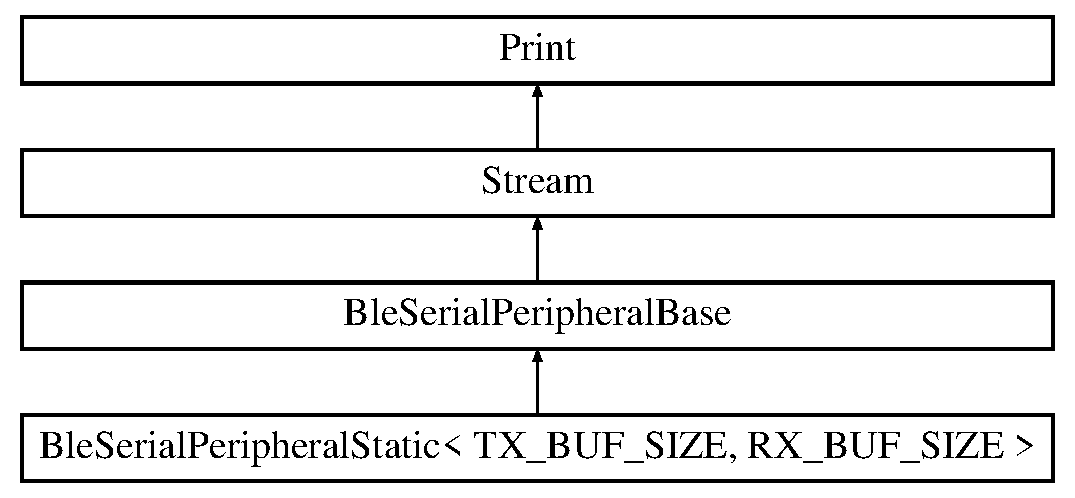
\includegraphics[height=4.000000cm]{class_stream}
\end{center}
\end{figure}
\subsection*{Public Member Functions}
\begin{DoxyCompactItemize}
\item 
virtual int \mbox{\hyperlink{class_stream_a9c98a763395005c08ce95afb2f06c7b1}{available}} ()=0
\begin{DoxyCompactList}\small\item\em Returns the number of a bytes available to read right now. \end{DoxyCompactList}\item 
virtual int \mbox{\hyperlink{class_stream_aea5dee9fcb038148515b7c9212d38dc0}{read}} ()=0
\begin{DoxyCompactList}\small\item\em Read a byte from the stream. \end{DoxyCompactList}\item 
virtual int \mbox{\hyperlink{class_stream_a30c3c212ec6ea67277a708c5ea2501a5}{peek}} ()=0
\begin{DoxyCompactList}\small\item\em Read a byte from the stream but do not remove it so read will return the same byte next time. \end{DoxyCompactList}\item 
\mbox{\Hypertarget{class_stream_aa3ef2c34f152a0b2ea8de9139b9461da}\label{class_stream_aa3ef2c34f152a0b2ea8de9139b9461da}} 
virtual void \mbox{\hyperlink{class_stream_aa3ef2c34f152a0b2ea8de9139b9461da}{flush}} ()=0
\begin{DoxyCompactList}\small\item\em For output streams, writes any unwritten buffered data. \end{DoxyCompactList}\item 
void \mbox{\hyperlink{class_stream_abaa50647d6dbb3baf7697a2691a06177}{set\+Timeout}} (system\+\_\+tick\+\_\+t timeout)
\begin{DoxyCompactList}\small\item\em Sets the read timeout (default\+: 1000 milliseconds) \end{DoxyCompactList}\item 
bool \mbox{\hyperlink{class_stream_a4bab30ccd324efd461dee46a2339f673}{find}} (char $\ast$target)
\begin{DoxyCompactList}\small\item\em Reads data from the stream until the target string is found. \end{DoxyCompactList}\item 
bool \mbox{\hyperlink{class_stream_ad851401f2318cdb1de05707e021b81d9}{find}} (char $\ast$target, size\+\_\+t length)
\begin{DoxyCompactList}\small\item\em Reads data from the stream until the target string is found. \end{DoxyCompactList}\item 
bool \mbox{\hyperlink{class_stream_ad1f5f6600832396fb38a897baf4de35b}{find\+Until}} (char $\ast$target, char $\ast$terminator)
\begin{DoxyCompactList}\small\item\em Reads data from the stream until the target string is found or the terminator string is found. \end{DoxyCompactList}\item 
bool \mbox{\hyperlink{class_stream_a3a9497de614792103ab8cb4759e01a69}{find\+Until}} (char $\ast$target, size\+\_\+t target\+Len, char $\ast$terminate, size\+\_\+t term\+Len)
\begin{DoxyCompactList}\small\item\em Reads data from the stream until the target string is found or the terminator string is found. \end{DoxyCompactList}\item 
long \mbox{\hyperlink{class_stream_a497ffcbcb4d5bb889a8fde487bcc1b98}{parse\+Int}} ()
\begin{DoxyCompactList}\small\item\em returns the first valid (long) integer value from the current position \end{DoxyCompactList}\item 
float \mbox{\hyperlink{class_stream_a5e5a0cc11eb586d89dcb7fa8e53a87e8}{parse\+Float}} ()
\begin{DoxyCompactList}\small\item\em returns the first valid float value from the current position \end{DoxyCompactList}\item 
size\+\_\+t \mbox{\hyperlink{class_stream_a45fd1336a323ea83b16e8507055f44ea}{read\+Bytes}} (char $\ast$buffer, size\+\_\+t length)
\begin{DoxyCompactList}\small\item\em Read chars from stream into buffer. \end{DoxyCompactList}\item 
size\+\_\+t \mbox{\hyperlink{class_stream_af84672a4fb2620466958d3118d4fea00}{read\+Bytes\+Until}} (char terminator, char $\ast$buffer, size\+\_\+t length)
\begin{DoxyCompactList}\small\item\em Read chars from stream into buffer until the character terminator is found. \end{DoxyCompactList}\item 
\mbox{\Hypertarget{class_stream_a1c60bdda2b65d78e5a1362d51b856c5a}\label{class_stream_a1c60bdda2b65d78e5a1362d51b856c5a}} 
String \mbox{\hyperlink{class_stream_a1c60bdda2b65d78e5a1362d51b856c5a}{read\+String}} ()
\begin{DoxyCompactList}\small\item\em Reads the remainder of the file into a string. \end{DoxyCompactList}\item 
String \mbox{\hyperlink{class_stream_a6a409da87c552909260d8cc428c5ca70}{read\+String\+Until}} (char terminator)
\begin{DoxyCompactList}\small\item\em Reads the remainder of the file into a string or until terminator is found. \end{DoxyCompactList}\end{DoxyCompactItemize}


\subsection{Detailed Description}
Arduino/\+Wiring \mbox{\hyperlink{class_stream}{Stream}} Class. 

Methods for reading data from a stream, such a serial port, T\+CP network stream, or a file. 

\subsection{Member Function Documentation}
\mbox{\Hypertarget{class_stream_a9c98a763395005c08ce95afb2f06c7b1}\label{class_stream_a9c98a763395005c08ce95afb2f06c7b1}} 
\index{Stream@{Stream}!available@{available}}
\index{available@{available}!Stream@{Stream}}
\subsubsection{\texorpdfstring{available()}{available()}}
{\footnotesize\ttfamily virtual int Stream\+::available (\begin{DoxyParamCaption}{ }\end{DoxyParamCaption})\hspace{0.3cm}{\ttfamily [pure virtual]}}



Returns the number of a bytes available to read right now. 

For files, the number of bytes left to read in the file from the current file position. 

Implemented in \mbox{\hyperlink{class_ble_serial_peripheral_base_a946cc56677f03db99de9409851427941}{Ble\+Serial\+Peripheral\+Base}}.

\mbox{\Hypertarget{class_stream_a4bab30ccd324efd461dee46a2339f673}\label{class_stream_a4bab30ccd324efd461dee46a2339f673}} 
\index{Stream@{Stream}!find@{find}}
\index{find@{find}!Stream@{Stream}}
\subsubsection{\texorpdfstring{find()}{find()}\hspace{0.1cm}{\footnotesize\ttfamily [1/2]}}
{\footnotesize\ttfamily bool Stream\+::find (\begin{DoxyParamCaption}\item[{char $\ast$}]{target }\end{DoxyParamCaption})}



Reads data from the stream until the target string is found. 


\begin{DoxyParams}{Parameters}
{\em target} & The string to search for (null-\/terminated c-\/string)\\
\hline
\end{DoxyParams}
\begin{DoxyReturn}{Returns}
true if target string is found, false if timed out (see set\+Timeout) 
\end{DoxyReturn}
\mbox{\Hypertarget{class_stream_ad851401f2318cdb1de05707e021b81d9}\label{class_stream_ad851401f2318cdb1de05707e021b81d9}} 
\index{Stream@{Stream}!find@{find}}
\index{find@{find}!Stream@{Stream}}
\subsubsection{\texorpdfstring{find()}{find()}\hspace{0.1cm}{\footnotesize\ttfamily [2/2]}}
{\footnotesize\ttfamily bool Stream\+::find (\begin{DoxyParamCaption}\item[{char $\ast$}]{target,  }\item[{size\+\_\+t}]{length }\end{DoxyParamCaption})}



Reads data from the stream until the target string is found. 


\begin{DoxyParams}{Parameters}
{\em target} & The string to search for. The string is specified by length so it does not need to be null-\/terminated.\\
\hline
{\em length} & The number of bytes in target to search for.\\
\hline
\end{DoxyParams}
\begin{DoxyReturn}{Returns}
true if target string is found, false if timed out (see set\+Timeout) 
\end{DoxyReturn}
\mbox{\Hypertarget{class_stream_ad1f5f6600832396fb38a897baf4de35b}\label{class_stream_ad1f5f6600832396fb38a897baf4de35b}} 
\index{Stream@{Stream}!find\+Until@{find\+Until}}
\index{find\+Until@{find\+Until}!Stream@{Stream}}
\subsubsection{\texorpdfstring{find\+Until()}{findUntil()}\hspace{0.1cm}{\footnotesize\ttfamily [1/2]}}
{\footnotesize\ttfamily bool Stream\+::find\+Until (\begin{DoxyParamCaption}\item[{char $\ast$}]{target,  }\item[{char $\ast$}]{terminator }\end{DoxyParamCaption})}



Reads data from the stream until the target string is found or the terminator string is found. 


\begin{DoxyParams}{Parameters}
{\em target} & The string to search for (null-\/terminated c-\/string)\\
\hline
{\em terminator} & The terminator string to search for (null-\/terminated c-\/string)\\
\hline
\end{DoxyParams}
\begin{DoxyReturn}{Returns}
true if target string is found, false if timed out (see set\+Timeout) 
\end{DoxyReturn}
\mbox{\Hypertarget{class_stream_a3a9497de614792103ab8cb4759e01a69}\label{class_stream_a3a9497de614792103ab8cb4759e01a69}} 
\index{Stream@{Stream}!find\+Until@{find\+Until}}
\index{find\+Until@{find\+Until}!Stream@{Stream}}
\subsubsection{\texorpdfstring{find\+Until()}{findUntil()}\hspace{0.1cm}{\footnotesize\ttfamily [2/2]}}
{\footnotesize\ttfamily bool Stream\+::find\+Until (\begin{DoxyParamCaption}\item[{char $\ast$}]{target,  }\item[{size\+\_\+t}]{target\+Len,  }\item[{char $\ast$}]{terminate,  }\item[{size\+\_\+t}]{term\+Len }\end{DoxyParamCaption})}



Reads data from the stream until the target string is found or the terminator string is found. 


\begin{DoxyParams}{Parameters}
{\em target} & The string to search for. The string is specified by length so it does not need to be null-\/terminated.\\
\hline
{\em length} & The number of bytes in target to search for.\\
\hline
{\em terminator} & The terminator string to search for. The string is specified by length so it does not need to be null-\/terminated.\\
\hline
{\em term\+Len} & The number of bytes in terminator to search for.\\
\hline
\end{DoxyParams}
\begin{DoxyReturn}{Returns}
true if target string is found, false if timed out (see set\+Timeout) 
\end{DoxyReturn}
\mbox{\Hypertarget{class_stream_a5e5a0cc11eb586d89dcb7fa8e53a87e8}\label{class_stream_a5e5a0cc11eb586d89dcb7fa8e53a87e8}} 
\index{Stream@{Stream}!parse\+Float@{parse\+Float}}
\index{parse\+Float@{parse\+Float}!Stream@{Stream}}
\subsubsection{\texorpdfstring{parse\+Float()}{parseFloat()}}
{\footnotesize\ttfamily float Stream\+::parse\+Float (\begin{DoxyParamCaption}{ }\end{DoxyParamCaption})}



returns the first valid float value from the current position 

Initial characters that are not digits (or the minus sign or .) are skipped float is terminated by the first character that is not a float character. Decimal part is separate by \textquotesingle{}.\textquotesingle{}. \mbox{\Hypertarget{class_stream_a497ffcbcb4d5bb889a8fde487bcc1b98}\label{class_stream_a497ffcbcb4d5bb889a8fde487bcc1b98}} 
\index{Stream@{Stream}!parse\+Int@{parse\+Int}}
\index{parse\+Int@{parse\+Int}!Stream@{Stream}}
\subsubsection{\texorpdfstring{parse\+Int()}{parseInt()}}
{\footnotesize\ttfamily long Stream\+::parse\+Int (\begin{DoxyParamCaption}{ }\end{DoxyParamCaption})}



returns the first valid (long) integer value from the current position 

Initial characters that are not digits (or the minus sign) are skipped integer is terminated by the first character that is not a digit. \mbox{\Hypertarget{class_stream_a30c3c212ec6ea67277a708c5ea2501a5}\label{class_stream_a30c3c212ec6ea67277a708c5ea2501a5}} 
\index{Stream@{Stream}!peek@{peek}}
\index{peek@{peek}!Stream@{Stream}}
\subsubsection{\texorpdfstring{peek()}{peek()}}
{\footnotesize\ttfamily virtual int Stream\+::peek (\begin{DoxyParamCaption}{ }\end{DoxyParamCaption})\hspace{0.3cm}{\ttfamily [pure virtual]}}



Read a byte from the stream but do not remove it so read will return the same byte next time. 

\begin{DoxyReturn}{Returns}
A byte value 0 -\/ 255, or -\/1 if there are no bytes available.
\end{DoxyReturn}
For files, the current file position is left unchanged. 

Implemented in \mbox{\hyperlink{class_ble_serial_peripheral_base_a6ba8319f3b1a69c96c4e8b3f8dde5bbc}{Ble\+Serial\+Peripheral\+Base}}.

\mbox{\Hypertarget{class_stream_aea5dee9fcb038148515b7c9212d38dc0}\label{class_stream_aea5dee9fcb038148515b7c9212d38dc0}} 
\index{Stream@{Stream}!read@{read}}
\index{read@{read}!Stream@{Stream}}
\subsubsection{\texorpdfstring{read()}{read()}}
{\footnotesize\ttfamily virtual int Stream\+::read (\begin{DoxyParamCaption}{ }\end{DoxyParamCaption})\hspace{0.3cm}{\ttfamily [pure virtual]}}



Read a byte from the stream. 

\begin{DoxyReturn}{Returns}
A byte value 0 -\/ 255, or -\/1 if there are no bytes available. 
\end{DoxyReturn}


Implemented in \mbox{\hyperlink{class_ble_serial_peripheral_base_a4933bc35d89028134597b46315806ce4}{Ble\+Serial\+Peripheral\+Base}}.

\mbox{\Hypertarget{class_stream_a45fd1336a323ea83b16e8507055f44ea}\label{class_stream_a45fd1336a323ea83b16e8507055f44ea}} 
\index{Stream@{Stream}!read\+Bytes@{read\+Bytes}}
\index{read\+Bytes@{read\+Bytes}!Stream@{Stream}}
\subsubsection{\texorpdfstring{read\+Bytes()}{readBytes()}}
{\footnotesize\ttfamily size\+\_\+t Stream\+::read\+Bytes (\begin{DoxyParamCaption}\item[{char $\ast$}]{buffer,  }\item[{size\+\_\+t}]{length }\end{DoxyParamCaption})}



Read chars from stream into buffer. 


\begin{DoxyParams}{Parameters}
{\em buffer} & The buffer to read into \\
\hline
{\em length} & The number of bytes to read \\
\hline
\end{DoxyParams}
\begin{DoxyReturn}{Returns}
the number of characters placed in the buffer (0 means no valid data found) 
\end{DoxyReturn}
\mbox{\Hypertarget{class_stream_af84672a4fb2620466958d3118d4fea00}\label{class_stream_af84672a4fb2620466958d3118d4fea00}} 
\index{Stream@{Stream}!read\+Bytes\+Until@{read\+Bytes\+Until}}
\index{read\+Bytes\+Until@{read\+Bytes\+Until}!Stream@{Stream}}
\subsubsection{\texorpdfstring{read\+Bytes\+Until()}{readBytesUntil()}}
{\footnotesize\ttfamily size\+\_\+t Stream\+::read\+Bytes\+Until (\begin{DoxyParamCaption}\item[{char}]{terminator,  }\item[{char $\ast$}]{buffer,  }\item[{size\+\_\+t}]{length }\end{DoxyParamCaption})}



Read chars from stream into buffer until the character terminator is found. 


\begin{DoxyParams}{Parameters}
{\em terminator} & The character to stop reading \\
\hline
{\em buffer} & The buffer to read into \\
\hline
{\em length} & The number of bytes to read \\
\hline
\end{DoxyParams}
\begin{DoxyReturn}{Returns}
the number of characters placed in the buffer (0 means no valid data found)
\end{DoxyReturn}
The terminator could be some thing like \textbackslash{}n (newline), \textbackslash{}t (tab), etc. depending on the data you are parsing. \mbox{\Hypertarget{class_stream_a6a409da87c552909260d8cc428c5ca70}\label{class_stream_a6a409da87c552909260d8cc428c5ca70}} 
\index{Stream@{Stream}!read\+String\+Until@{read\+String\+Until}}
\index{read\+String\+Until@{read\+String\+Until}!Stream@{Stream}}
\subsubsection{\texorpdfstring{read\+String\+Until()}{readStringUntil()}}
{\footnotesize\ttfamily String Stream\+::read\+String\+Until (\begin{DoxyParamCaption}\item[{char}]{terminator }\end{DoxyParamCaption})}



Reads the remainder of the file into a string or until terminator is found. 


\begin{DoxyParams}{Parameters}
{\em terminator} & The character to stop reading at. \\
\hline
\end{DoxyParams}
\mbox{\Hypertarget{class_stream_abaa50647d6dbb3baf7697a2691a06177}\label{class_stream_abaa50647d6dbb3baf7697a2691a06177}} 
\index{Stream@{Stream}!set\+Timeout@{set\+Timeout}}
\index{set\+Timeout@{set\+Timeout}!Stream@{Stream}}
\subsubsection{\texorpdfstring{set\+Timeout()}{setTimeout()}}
{\footnotesize\ttfamily void Stream\+::set\+Timeout (\begin{DoxyParamCaption}\item[{system\+\_\+tick\+\_\+t}]{timeout }\end{DoxyParamCaption})}



Sets the read timeout (default\+: 1000 milliseconds) 

This makes more sense for network and serial streams. 

The documentation for this class was generated from the following file\+:\begin{DoxyCompactItemize}
\item 
docs/src/\mbox{\hyperlink{spark__wiring__stream_8h}{spark\+\_\+wiring\+\_\+stream.\+h}}\end{DoxyCompactItemize}

\chapter{File Documentation}
\hypertarget{spark__wiring__print_8h}{}\section{docs/src/spark\+\_\+wiring\+\_\+print.h File Reference}
\label{spark__wiring__print_8h}\index{docs/src/spark\+\_\+wiring\+\_\+print.\+h@{docs/src/spark\+\_\+wiring\+\_\+print.\+h}}


Header for spark\+\_\+wiring\+\_\+print.\+c module.  


{\ttfamily \#include $<$stddef.\+h$>$}\newline
{\ttfamily \#include $<$string.\+h$>$}\newline
{\ttfamily \#include $<$stdint.\+h$>$}\newline
{\ttfamily \#include \char`\"{}spark\+\_\+wiring\+\_\+string.\+h\char`\"{}}\newline
{\ttfamily \#include \char`\"{}spark\+\_\+wiring\+\_\+printable.\+h\char`\"{}}\newline
\subsection*{Data Structures}
\begin{DoxyCompactItemize}
\item 
class \mbox{\hyperlink{class_print}{Print}}
\begin{DoxyCompactList}\small\item\em Class for printing to a stream or file. \end{DoxyCompactList}\end{DoxyCompactItemize}
\subsection*{Variables}
\begin{DoxyCompactItemize}
\item 
\mbox{\Hypertarget{spark__wiring__print_8h_a26e216c38cffa0a9965fa7933ba558b1}\label{spark__wiring__print_8h_a26e216c38cffa0a9965fa7933ba558b1}} 
const unsigned char {\bfseries D\+EC} = 10
\item 
\mbox{\Hypertarget{spark__wiring__print_8h_a777726851dda95dabcc50f606e2dfd8e}\label{spark__wiring__print_8h_a777726851dda95dabcc50f606e2dfd8e}} 
const unsigned char {\bfseries H\+EX} = 16
\item 
\mbox{\Hypertarget{spark__wiring__print_8h_aeea5c9efade0b29d08f3b5b8336425ad}\label{spark__wiring__print_8h_aeea5c9efade0b29d08f3b5b8336425ad}} 
const unsigned char {\bfseries O\+CT} = 8
\item 
\mbox{\Hypertarget{spark__wiring__print_8h_aee179d58d1b76a9b42397af886f2f9a4}\label{spark__wiring__print_8h_aee179d58d1b76a9b42397af886f2f9a4}} 
const unsigned char {\bfseries B\+IN} = 2
\end{DoxyCompactItemize}


\subsection{Detailed Description}
Header for spark\+\_\+wiring\+\_\+print.\+c module. 

\begin{DoxyAuthor}{Author}
Mohit Bhoite 
\end{DoxyAuthor}
\begin{DoxyVersion}{Version}
V1.\+0.\+0 
\end{DoxyVersion}
\begin{DoxyDate}{Date}
13-\/\+March-\/2013 Copyright (c) 2013-\/2015 Particle Industries, Inc. All rights reserved. Copyright (c) 2010 David A. Mellis. All right reserved.
\end{DoxyDate}
This library is free software; you can redistribute it and/or modify it under the terms of the G\+NU Lesser General Public License as published by the Free Software Foundation, either version 3 of the License, or (at your option) any later version.

This library is distributed in the hope that it will be useful, but W\+I\+T\+H\+O\+UT A\+NY W\+A\+R\+R\+A\+N\+TY; without even the implied warranty of M\+E\+R\+C\+H\+A\+N\+T\+A\+B\+I\+L\+I\+TY or F\+I\+T\+N\+E\+SS F\+OR A P\+A\+R\+T\+I\+C\+U\+L\+AR P\+U\+R\+P\+O\+SE. See the G\+NU Lesser General Public License for more details.

You should have received a copy of the G\+NU Lesser General Public License along with this library; if not, see \href{http://www.gnu.org/licenses/}{\tt http\+://www.\+gnu.\+org/licenses/}. 
\hypertarget{spark__wiring__stream_8h}{}\section{docs/src/spark\+\_\+wiring\+\_\+stream.h File Reference}
\label{spark__wiring__stream_8h}\index{docs/src/spark\+\_\+wiring\+\_\+stream.\+h@{docs/src/spark\+\_\+wiring\+\_\+stream.\+h}}


Header for spark\+\_\+wiring\+\_\+stream.\+c module.  


{\ttfamily \#include \char`\"{}spark\+\_\+wiring\+\_\+string.\+h\char`\"{}}\newline
{\ttfamily \#include \char`\"{}spark\+\_\+wiring\+\_\+print.\+h\char`\"{}}\newline
{\ttfamily \#include \char`\"{}system\+\_\+tick\+\_\+hal.\+h\char`\"{}}\newline
\subsection*{Data Structures}
\begin{DoxyCompactItemize}
\item 
class \mbox{\hyperlink{class_stream}{Stream}}
\begin{DoxyCompactList}\small\item\em Arduino/\+Wiring \mbox{\hyperlink{class_stream}{Stream}} Class. \end{DoxyCompactList}\end{DoxyCompactItemize}


\subsection{Detailed Description}
Header for spark\+\_\+wiring\+\_\+stream.\+c module. 

\begin{DoxyAuthor}{Author}
Mohit Bhoite 
\end{DoxyAuthor}
\begin{DoxyVersion}{Version}
V1.\+0.\+0 
\end{DoxyVersion}
\begin{DoxyDate}{Date}
13-\/\+March-\/2013 Copyright (c) 2013-\/2015 Particle Industries, Inc. All rights reserved. Copyright (c) 2010 David A. Mellis. All right reserved.
\end{DoxyDate}
This library is free software; you can redistribute it and/or modify it under the terms of the G\+NU Lesser General Public License as published by the Free Software Foundation, either version 3 of the License, or (at your option) any later version.

This library is distributed in the hope that it will be useful, but W\+I\+T\+H\+O\+UT A\+NY W\+A\+R\+R\+A\+N\+TY; without even the implied warranty of M\+E\+R\+C\+H\+A\+N\+T\+A\+B\+I\+L\+I\+TY or F\+I\+T\+N\+E\+SS F\+OR A P\+A\+R\+T\+I\+C\+U\+L\+AR P\+U\+R\+P\+O\+SE. See the G\+NU Lesser General Public License for more details.

You should have received a copy of the G\+NU Lesser General Public License along with this library; if not, see \href{http://www.gnu.org/licenses/}{\tt http\+://www.\+gnu.\+org/licenses/}. 
%--- End generated contents ---

% Index
\backmatter
\newpage
\phantomsection
\clearemptydoublepage
\addcontentsline{toc}{chapter}{Index}
\printindex

\end{document}
